\documentclass[10pt,journal,compsoc]{IEEEtran}

\usepackage{cite}
\usepackage{amsmath,amssymb,amsfonts}
\usepackage{graphicx}
\usepackage{textcomp}
\usepackage{booktabs}
\usepackage{multirow}
\usepackage{url}
\usepackage{hyperref}
\usepackage{xcolor}
\usepackage{siunitx}

\graphicspath{{figures/}}

\begin{document}

\title{Speculative GHR Forwarding: Eliminating Stale Branch-Predictor State in Deep FPGA Pipelines}

\author{
\IEEEauthorblockN{Devansh Joshi}
\IEEEauthorblockA{Department of Electrical and Computer Engineering\\
Email: devanshjoshi08@gmail.com}
}

\maketitle

\begin{abstract}
Deep pipelines on FPGA fabric suffer a branch-prediction degradation that has not been isolated under controlled conditions: the global history register (GHR) becomes stale as update latency grows with pipeline depth, inflating misprediction counts even when predictor hardware is unchanged.
Using five RV32IM pipeline variants (4 through 8 stages) synthesized from shared RTL on Xilinx Artix-7, we separate pipeline-depth CPI overhead into two mechanisms: Mechanism~A (longer per-misprediction flush penalty, inherent to depth) and Mechanism~B (inflated misprediction count from stale GHR state, correctable).
To eliminate Mechanism~B, we propose Speculative GHR Forwarding (SGF), a dual-GHR architecture that speculatively updates the history register at prediction time with checkpoint-based rollback.
SGF reduces mispredictions by up to 31\% on branch-dense workloads at 0.5--0.7\% area cost with no frequency degradation.
A first-principles CPI model ($R^2 = 0.977$, 35 data points) and 50 post-place-and-route synthesis runs with full statistical analysis support the measurements.
\end{abstract}

\begin{IEEEkeywords}
RISC-V, pipeline depth, FPGA, Artix-7, RV32IM, branch prediction, gshare, speculative GHR forwarding, microarchitecture
\end{IEEEkeywords}

% ====================================================================
\section{Introduction}
\label{sec:intro}
% ====================================================================

How deep should an FPGA pipeline be?
On ASIC processes the answer is well studied: partition the datapath until gate delay per stage reaches 6--8 FO4 inverter delays, then stop because branch-misprediction penalties and power begin to dominate \cite{hrishikesh2002optimal, sprangle2002increasing}.
On FPGAs, where LUT delay is largely function-independent and routing delay dominates timing \cite{xilinx_7series, boutros2020fpga, kuon2007measuring}, that answer does not transfer.
To our knowledge, no published study isolates pipeline depth as the sole independent variable on a common FPGA target while holding all other microarchitectural modules constant at the RTL level.
Prior RISC-V soft cores differ in ISA support, predictor design, memory architecture, and forwarding strategy, making performance differences across projects unattributable to any single factor.

As soft cores increasingly replace fixed-function IP in edge computing, embedded signal processing, and domain-specific accelerator control paths, understanding the limits of deep in-order pipelining on FPGAs becomes a systems-level question, not a niche academic exercise.

A less visible cost of deep pipelines compounds the problem.
In a deeper pipeline, the latency between branch resolution and the next prediction spans more cycles.
During these cycles the predictor's global history register (GHR) operates on stale state: branches predicted before prior branches resolve use a GHR that does not reflect the most recent outcomes.
Gonzalez and Horowitz identified this effect in ASIC power-performance simulations \cite{gonzalez1999power}, and high-performance ASIC out-of-order processors (e.g., Alpha~21264, MIPS~R10000) deploy speculative history update mechanisms to address it.
However, those mechanisms rely on deep reorder buffers, checkpoint arrays, and aggressive clock trees that are impractical on resource-constrained FPGA fabric.
To our knowledge, this effect has not been measured on FPGA fabric, where the pipeline-depth landscape differs fundamentally from ASIC and where a lightweight, in-order-compatible solution is needed.

This paper provides two things the literature lacks.
First, we build a controlled experiment: five RV32IM pipeline variants (4, 5, 6, 7, and 8 stages) that share identical RTL for the ALU, multiply-divide unit, gshare branch predictor, CSR unit, register file, instruction cache, and data memory.
Only pipeline interconnect, forwarding, and hazard detection differ.
We synthesize all five on Xilinx Artix-7 XC7A35T with 10 placement seeds per variant (50 runs total), run seven benchmark workloads from three standard sources, and collect 35 validated workload--depth data points.
Second, we separate the CPI cost of deeper pipelining into two mechanisms and eliminate the correctable one:

\begin{itemize}
\item \textbf{Mechanism~A:} Higher per-misprediction flush penalty (more stages to drain). Present on all workloads, predictable from pipeline structure.
\item \textbf{Mechanism~B:} Inflated misprediction count from stale GHR state. Present on branch-dense workloads (+5.7\% on CoreMark, +10\% on statemate at deeper pipelines). Unpredictable without simulation.
\end{itemize}

The key finding is a two-tier $F_{\max}$ structure on Artix-7: shallow pipelines (4/5-stage) cluster at 70--74\,MHz, while deep pipelines (6/7/8-stage) cluster at 115--118\,MHz ($p < 10^{-48}$, Cohen's $d = 18.5$).
On this Artix-7 fabric, the execute-stage split at depth~6 is the only statistically significant frequency knee observed ($p < 10^{-48}$).
Within each tier, additional stages buy no frequency.

Mechanism~A is inherent to pipeline depth and cannot be eliminated without reducing the pipeline.
Mechanism~B is a correctable deficiency in the predictor's update path.
Speculative history updates are well established in complex ASIC out-of-order processors (e.g., Alpha~21264, MIPS~R10000), but those mechanisms rely on deep reorder buffers and aggressive clock trees impractical on FPGA fabric.
SGF is, to our knowledge, the first dual-GHR checkpointing architecture designed for resource-constrained, in-order soft-core processors on LUT-based FPGA.
Speculative GHR Forwarding (SGF) balances the rigid routing constraints of LUT-based interconnects without inducing frequency degradation.
Measured results on Artix-7 show that SGF reduces mispredictions by 31.4\% on CoreMark and 22.7\% on statemate in 7-stage pipelines, at a cost of 55 LUTs and 63 flip-flops (0.7\% area) with no $F_{\max}$ loss.

A surprising result: SGF pushes 7/8-stage misprediction counts \emph{below} the 4/5-stage baseline (101K vs.\ 145K on CoreMark).
The speculative GHR is more accurate than a committed GHR at any pipeline depth because it reflects the most recent predicted control flow rather than waiting for resolution.

The contributions of this work are:
\begin{enumerate}
    \item \textbf{Speculative GHR Forwarding (SGF):} a lightweight dual-GHR mechanism that eliminates stale-GHR misprediction inflation (Mechanism~B) in deep FPGA pipelines, reducing mispredictions by up to 31.4\% at 0.5--0.7\% area cost with no $F_{\max}$ loss (Section~\ref{sec:sgf}).
    \item \textbf{First FPGA measurement of stale-GHR degradation:} controlled separation of pipeline-depth CPI overhead into Mechanism~A (penalty scaling) and Mechanism~B (stale-GHR misprediction inflation), with per-workload classification across seven benchmarks (Section~\ref{sec:mispred}).
    \item \textbf{Analytical CPI model:} a first-principles decomposition achieving $R^2 = 0.977$ across 35 workload--depth data points, with physically interpretable terms for branch flush, load-use stalls, and IF2 bubbles (Section~\ref{sec:model}).
    \item \textbf{Controlled experimental methodology:} pipeline depth as the sole independent variable across five design points, with all other microarchitectural modules shared from a common RTL codebase (Section~\ref{sec:methodology}).
    \item \textbf{Multi-seed FPGA characterization:} 50 post-place-and-route runs establishing a two-tier frequency structure with full statistical analysis (Section~\ref{sec:synth}).
\end{enumerate}

% ====================================================================
\section{Background and Related Work}
\label{sec:background}
% ====================================================================

\subsection{RISC-V ISA}

The RISC-V specification defines a modular instruction set with a base integer set (RV32I) and optional extensions \cite{waterman2019riscv}.
The M extension adds hardware multiply and divide instructions.
Together, RV32IM provides a complete integer computation substrate for embedded processors.
The fixed 32-bit instruction encoding and regular register-operand fields simplify decode logic and make the ISA well suited for pipelined implementation \cite{patterson2020computer}.

\subsection{Pipeline Depth Tradeoffs}

A pipelined processor overlaps execution of multiple instructions by partitioning the datapath into sequential stages separated by pipeline registers \cite{hennessy2017computer, patterson1985reduced}.
Deeper pipelines reduce the combinational logic between registers, potentially increasing clock frequency.
However, each additional stage increases the branch misprediction penalty by one cycle, adds pipeline register area and power, and introduces additional forwarding paths \cite{hrishikesh2002optimal}.

Hrishikesh et al.\ established that the optimal pipeline depth for ASIC designs is 6--8 FO4 inverter delays per stage \cite{hrishikesh2002optimal}.
Sprangle and Carmean analyzed the performance returns of deeper pipelines on superscalar architectures and showed diminishing returns beyond certain depths \cite{sprangle2002increasing}.
Both studies assume ASIC timing characteristics where gate delay scales linearly with logic depth.

A less commonly discussed effect is the impact on branch prediction accuracy itself.
In a deeper pipeline, the latency from branch execution (where the prediction is verified) back to the fetch stage (where the prediction is consumed) spans more cycles.
During these cycles, the predictor operates on stale state.
If two branches are closely spaced in the instruction stream, the second branch may be fetched and predicted before the first branch's outcome has updated the PHT.
Gonzalez and Horowitz identified this effect in the context of ASIC power-performance analysis \cite{gonzalez1999power}, but it has never been measured on FPGA fabric.

\subsection{FPGA Architecture Considerations}

Xilinx 7-series FPGAs implement combinational logic in 6-input LUTs grouped into configurable logic blocks \cite{xilinx_7series}.
Unlike ASIC standard cells, LUT delay is largely independent of the function implemented: a 6-input AND and a 6-input parity check have the same propagation delay through the LUT.
Routing delay, which depends on placement and the programmable interconnect, often exceeds LUT delay and is less predictable at design time \cite{boutros2020fpga}.
DSP48E1 hard blocks provide registered multiply-accumulate with fixed pipeline latency.
Block RAM offers single-cycle synchronous read with registered output.

These fabric properties mean that splitting a combinational path across two pipeline stages may not yield the same frequency improvement as on an ASIC.
Inserting a register does not eliminate the routing delay on either side of the register.
The frequency benefit of deeper pipelining on FPGA depends on whether the split targets a path dominated by LUT delay (effective) or routing delay (ineffective) \cite{kuon2007measuring}.

\subsection{Related RISC-V Soft Cores}

Table~\ref{tab:prior} summarizes the experimental scope of prior RISC-V FPGA implementations.
SERV \cite{serv2019} uses bit-serial execution (one stage, $\sim$300\,MHz on Artix-7).
PicoRV32 \cite{picorv32} uses multi-cycle execution without pipelining ($\sim$250\,MHz).
VexRiscv \cite{vexriscv} offers a highly configurable pipeline with optional branch prediction, caches, and MMU, but its pipeline depth cannot be varied independently of other features.
Ibex \cite{schiavone2017slow} is a 2-stage design targeting ultra-low power.
CVA6 \cite{zaruba2019ariane} implements RV64GC with a 6-stage pipeline and out-of-order commit.
SweRV EH1 \cite{swerv2019} is a commercial-grade 2-wide superscalar.
None of these projects provides a controlled comparison across pipeline depths with invariant predictor, MDU, and memory hardware.

The branch-prediction update-latency problem is well characterized in the ASIC literature.
Gonzalez and Horowitz \cite{gonzalez1999power} showed that deeper ASIC pipelines degrade predictor accuracy through increased feedback delay.
Seznec and Michaud studied the interaction between predictor update latency and table aliasing in tournament and TAGE predictors.
Speculative history update mechanisms are standard in high-performance ASIC out-of-order processors (Alpha~21264, MIPS~R10000), where deep reorder buffers provide checkpoint storage.
On FPGA soft cores, where area and routing constraints preclude reorder buffers, these techniques have not been adapted.
Our SGF mechanism addresses this gap with a lightweight, in-order-compatible design.

Prior surveys have cataloged pipelining techniques across RISC families \cite{biglari2019pipelining}, and the Rocket Chip generator \cite{asanovic2016rocket} offers a configurable pipeline, but neither isolates pipeline depth as a controlled variable or addresses the stale-GHR effect on FPGA fabric.

\begin{table*}[t]
\centering
\caption{Comparison of experimental scope with prior RISC-V FPGA implementations. \checkmark\ = varied; -- = fixed or not applicable.}
\label{tab:prior}
\small
\begin{tabular}{@{}lcccccc@{}}
\toprule
 & \rotatebox{70}{Pipeline depth} & \rotatebox{70}{Predictor} & \rotatebox{70}{ISA subset} & \rotatebox{70}{Memory type} & \rotatebox{70}{Forwarding} & \rotatebox{70}{Controlled} \\
\midrule
SERV \cite{serv2019}         & --  & --  & -- & -- & -- & -- \\
PicoRV32 \cite{picorv32}     & --  & --  & -- & -- & -- & -- \\
VexRiscv \cite{vexriscv}     & \checkmark & \checkmark & \checkmark & -- & \checkmark & -- \\
Ibex \cite{schiavone2017slow}& --  & --  & -- & -- & -- & -- \\
CVA6 \cite{zaruba2019ariane} & --  & --  & -- & -- & -- & -- \\
SweRV \cite{swerv2019}       & --  & --  & -- & -- & -- & -- \\
Rocket \cite{asanovic2016rocket} & \checkmark & \checkmark & \checkmark & \checkmark & \checkmark & -- \\
\textbf{This work}           & \checkmark & -- & -- & \checkmark & -- & \checkmark \\
\bottomrule
\end{tabular}
\vspace{2pt}

\footnotesize{``Controlled'' = only the indicated variable changes; all others are held constant from shared RTL.}
\end{table*}

The gap is not the absence of pipeline-depth variation per se, but the absence of a controlled experiment in which \emph{only} pipeline depth varies while all other microarchitectural variables are held constant on the same FPGA device---and the absence of any mechanism to correct the stale-GHR degradation that such an experiment reveals.

% ====================================================================
\section{Experimental Setup}
\label{sec:methodology}
% ====================================================================

\subsection{Common Microarchitecture}
\label{sec:common}

All five pipeline variants share the following modules, instantiated from identical RTL source files:

\textbf{ALU.} A combinational 10-operation arithmetic logic unit supporting ADD, SUB, AND, OR, XOR, SLT, SLTU, SLL, SRL, and SRA.

\textbf{Multiply-Divide Unit (MDU).} A 2-cycle pipelined multiplier with registered input and output stages, designed to infer DSP48E1 blocks. The divider uses a 32-cycle restoring algorithm. Supported operations are MUL, MULH, MULHSU, MULHU, DIV, DIVU, REM, and REMU. Division by zero and signed overflow follow the RISC-V specification \cite{waterman2019riscv}.

\textbf{Branch Predictor.} A gshare predictor \cite{mcfarling1993combining} with a 64-entry pattern history table (PHT) of 2-bit saturating counters, a 6-bit global history register (GHR), a 32-entry direct-mapped branch target buffer (BTB), and a 4-entry return address stack (RAS). The PHT is indexed by XORing the lower PC bits with the GHR. The predictor hardware is identical in all five variants. However, the number of pipeline stages between the fetch stage (where predictions are made) and the execute stage (where predictions are resolved and the PHT is updated) differs across variants. This update latency is the central variable in our analysis and the target of SGF.

\textbf{CSR Unit.} Machine-mode control and status registers including \texttt{mstatus}, \texttt{mtvec}, \texttt{mepc}, \texttt{mcause}, \texttt{mscratch}, and 64-bit hardware performance counters for cycles (\texttt{mcycle}), retired instructions (\texttt{minstret}), total branches, and branch mispredictions. Each benchmark reads these counters to obtain cycle counts, instruction counts, branch counts, and misprediction counts.

\textbf{Instruction Memory.} A 1024-word (4\,KB) ROM initialized at elaboration via \texttt{\$readmemh}. A 64-line direct-mapped instruction cache with combinational hit logic sits between the PC and the instruction memory.

\textbf{Data Memory.} A 1024-word (4\,KB) synchronous RAM supporting byte, halfword, and word loads (signed and unsigned) and stores.

\textbf{Register File.} A 32$\times$32-bit register file with two read ports and one write port, including a write-through bypass for simultaneous read and write to the same register.

\subsection{Pipeline Variants}
\label{sec:variants}

The five variants are constructed by splitting or merging stages of a common datapath.
Each split targets a specific combinational path:

\textbf{4-stage} (IF, ID, EX, MEM/WB): Merges memory access and write-back, eliminating load-use hazards but creating the longest critical path. One forwarding source (MEM/WB$\to$EX). Branch penalty: 2 cycles.

\textbf{5-stage} (IF, ID, EX, MEM, WB): Classic RISC organization \cite{patterson1985reduced}. Introduces a 1-cycle load-use stall. Two forwarding sources. Branch penalty: 2 cycles.

\textbf{6-stage} (IF, ID, EX1, EX2, MEM, WB): Splits the execute phase, separating the forwarding multiplexer (EX1) from ALU and branch comparator (EX2). Three forwarding sources. Branch penalty: 3 cycles. This split targets the dominant critical path in the 4/5-stage designs.

\textbf{7-stage} (IF1, IF2, ID, EX1, EX2, MEM, WB): Splits instruction fetch, placing branch prediction in IF2 with a registered PC. Introduces a 1-cycle IF2 bubble on every correctly predicted taken branch (IF1's speculative fetch is discarded). Branch penalty: 4 cycles. This split targets BRAM read latency. An industrial pipeline might deploy a zero-delay Next-Line Predictor (NLP) or BTB directly in IF1 to eliminate this bubble; we do not, because embedding specialized routing paths in IF1 would alter the physical timing paths unevenly across the 4-to-8-stage variants. The bubble is a deliberate control-variable constraint that preserves strict structural invariants across all depths.

\textbf{8-stage} (IF1, IF2, ID, EX1, EX2, MEM1, MEM2, WB): Splits memory access, creating a dual load-use stall (loads not available until MEM2). Branch penalty: 4 cycles.

Table~\ref{tab:hazard} summarizes the per-event costs.
The 7/8-stage variants share the same branch penalty because both resolve branches in EX2 with equal numbers of preceding stages.
The predictor update latency---the number of stages between prediction and resolution---is the critical parameter for Mechanism~B.

\begin{table*}[t]
\centering
\caption{Hazard handling comparison across pipeline depths.}
\label{tab:hazard}
\begin{tabular}{@{}lccccc@{}}
\toprule
\textbf{Property} & \textbf{4-stg} & \textbf{5-stg} & \textbf{6-stg} & \textbf{7-stg} & \textbf{8-stg} \\
\midrule
Pipeline registers        & 3 & 4 & 5 & 6 & 7 \\
Forwarding sources        & 1 & 2 & 3 & 3 & 3 \\
Load-use stall            & 0 & 1\,cy & 1\,cy & 1\,cy & 1--2\,cy \\
Branch penalty            & 2\,cy & 2\,cy & 3\,cy & 4\,cy & 4\,cy \\
IF2 prediction bubble     & -- & -- & -- & 1\,cy & 1\,cy \\
Predictor update latency  & 2 & 2 & 3 & 4 & 4 \\
\bottomrule
\end{tabular}
\end{table*}

\subsection{Synthesis Methodology}
\label{sec:synth_method}

To quantify placement-dependent variance in $F_{\max}$, each variant is synthesized and implemented 10 times with different placement and routing directive combinations (Default, Explore, ExtraNetDelay\_high/low, ExtraPostPlacementOpt, NoTimingRelaxation, and AggressiveExplore in various pairings).
This produces 50 independent implementation runs (5 variants $\times$ 10 seeds).
The target device is Xilinx Artix-7 XC7A35TCPG236-1.
All syntheses use Vivado 2025.2 in out-of-context (OOC) mode with a 5\,ns clock constraint (200\,MHz target) to drive the tools toward maximum optimization effort.
The reported $F_{\max}$ values are means with standard deviations and 95\% confidence intervals computed via Student's $t$-distribution with 9 degrees of freedom.
$F_{\max}$ for each run is derived from the worst negative slack (WNS) as $F_{\max} = 1000/(5 - \text{WNS})$.

\textbf{Reproducibility.}
All benchmarks are compiled with \texttt{riscv-none-elf-gcc}~15.2.0 (xPack) using \texttt{-march=rv32im\_zicsr -mabi=ilp32 -O1 -nostdlib -ffreestanding}.
CoreMark uses the official EEMBC source (\texttt{github.com/eembc/coremark}) with a bare-metal porting layer; Embench-IoT uses the official source (\texttt{github.com/embench/embench-iot}).
Linker scripts place code at address 0 (IMEM) and data at 0x10000 (DMEM); the startup routine clears BSS and initializes seed variables before calling \texttt{main}.
The 10 placement/routing directive pairings are: (1)~Default/Default, (2)~Explore/Explore, (3)~Default/NoTimingRelaxation, (4)~ExtraNetDelay\_high/Explore, (5)~Default/Default, (6)~ExtraPostPlacementOpt/AggressiveExplore, (7)~Explore/NoTimingRelaxation, (8)~ExtraNetDelay\_low/Explore, (9)~Default/AggressiveExplore, (10)~Explore/NoTimingRelaxation.
Complete RTL, synthesis TCL scripts, benchmark hex files, and result logs are archived at \texttt{github.com/devanshjoshi08/RISCV-Pipeline-Research}.

\subsection{Benchmark Suite}
\label{sec:benchmarks}

Seven workloads from three standard sources measure CPI and branch prediction behavior across all five depths.
Each benchmark reads the hardware performance counters (\texttt{mcycle}, \texttt{minstret}, branch count, misprediction count) before and after the workload, computes deltas, and stores results to data memory for testbench readout.
Functional correctness is verified by confirming that all five pipeline variants produce identical instruction counts, branch counts, and memory checksums for each workload.

\textbf{Dhrystone 2.1.} A synthetic integer benchmark \cite{hennessy2017computer} ported to bare-metal RV32IM: 100 iterations, 2{,}926 instructions, 400 branches (13.7\% branch frequency).

\textbf{Diagnostic workload.} A mixed program exercising integer arithmetic, load/store sequences, function calls, and conditional branches: 1{,}367 instructions, 360 branches (26.3\% branch frequency).

\textbf{Official EEMBC CoreMark.} The industry-standard CoreMark benchmark \cite{coremark}, compiled from the official EEMBC source using riscv-none-elf-gcc~15.2.0 with -O1 optimization: 10 iterations in PERFORMANCE\_RUN mode, 2{,}893{,}145 instructions, 719{,}810 branches (24.9\% branch frequency).

\textbf{Embench-IoT: aha-mont64.} Montgomery multiplication from the official Embench-IoT suite. Cryptographic kernel, multiply-heavy: 4{,}453{,}858 instructions, 512{,}593 branches (11.5\%).

\textbf{Embench-IoT: crc32.} CRC-32 computation: 4{,}008{,}648 instructions, 174{,}591 branches (4.4\%). Inner loop has extremely predictable branching (0.19\% misprediction rate).

\textbf{Embench-IoT: statemate.} Finite state machine simulation: 3{,}160{,}225 instructions, 376{,}291 branches (11.9\%). Data-dependent state transitions produce a moderate misprediction rate that increases with pipeline depth.

\textbf{Embench-IoT: edn.} Encoder-decoder signal processing: 2{,}972{,}527 instructions, 338{,}986 branches (11.4\%).

% ====================================================================
\section{Baseline Results}
\label{sec:results}
% ====================================================================

This section establishes the baseline measurements that motivate SGF.
The synthesis results reveal the FPGA-specific frequency structure; the CPI measurements expose Mechanism~B as the target for correction.

\subsection{Synthesis Results}
\label{sec:synth}

Table~\ref{tab:results} presents the post-place-and-route results for all five variants.
Fig.~\ref{fig:fmax} shows the frequency comparison with error bars.

\begin{table*}[t]
\centering
\caption{Post-place-and-route synthesis results on Artix-7 XC7A35T (mean $\pm$ std from 10 placement seeds, 50 runs total). 95\% confidence intervals computed via Student's $t$ with 9 d.f. Tier gap: two-sample $t$-test $p < 10^{-48}$, Cohen's $d = 18.5$.}
\label{tab:results}
\begin{tabular}{@{}lccccc@{}}
\toprule
\textbf{Metric} & \textbf{4-stg} & \textbf{5-stg} & \textbf{6-stg} & \textbf{7-stg} & \textbf{8-stg} \\
\midrule
$F_{\max}$ (MHz)  & 70.4  & 74.0  & 117.3  & 115.0  & 117.5 \\
$\pm$ std (MHz)   & 2.4   & 1.5   & 1.4    & 2.0    & 1.8 \\
95\% CI (MHz)     & [68.7, 72.1] & [72.9, 75.1] & [116.3, 118.3] & [113.5, 116.5] & [116.2, 118.8] \\
Slice LUTs        & 7{,}219 & 7{,}429 & 7{,}631 & 7{,}766 & 7{,}841 \\
Slice Regs (FFs)  & 8{,}040 & 8{,}190 & 8{,}501 & 8{,}550 & 8{,}678 \\
DSP48E1           & 12    & 12     & 12     & 12     & 12 \\
\bottomrule
\end{tabular}
\end{table*}

\begin{figure}[t]
\centering
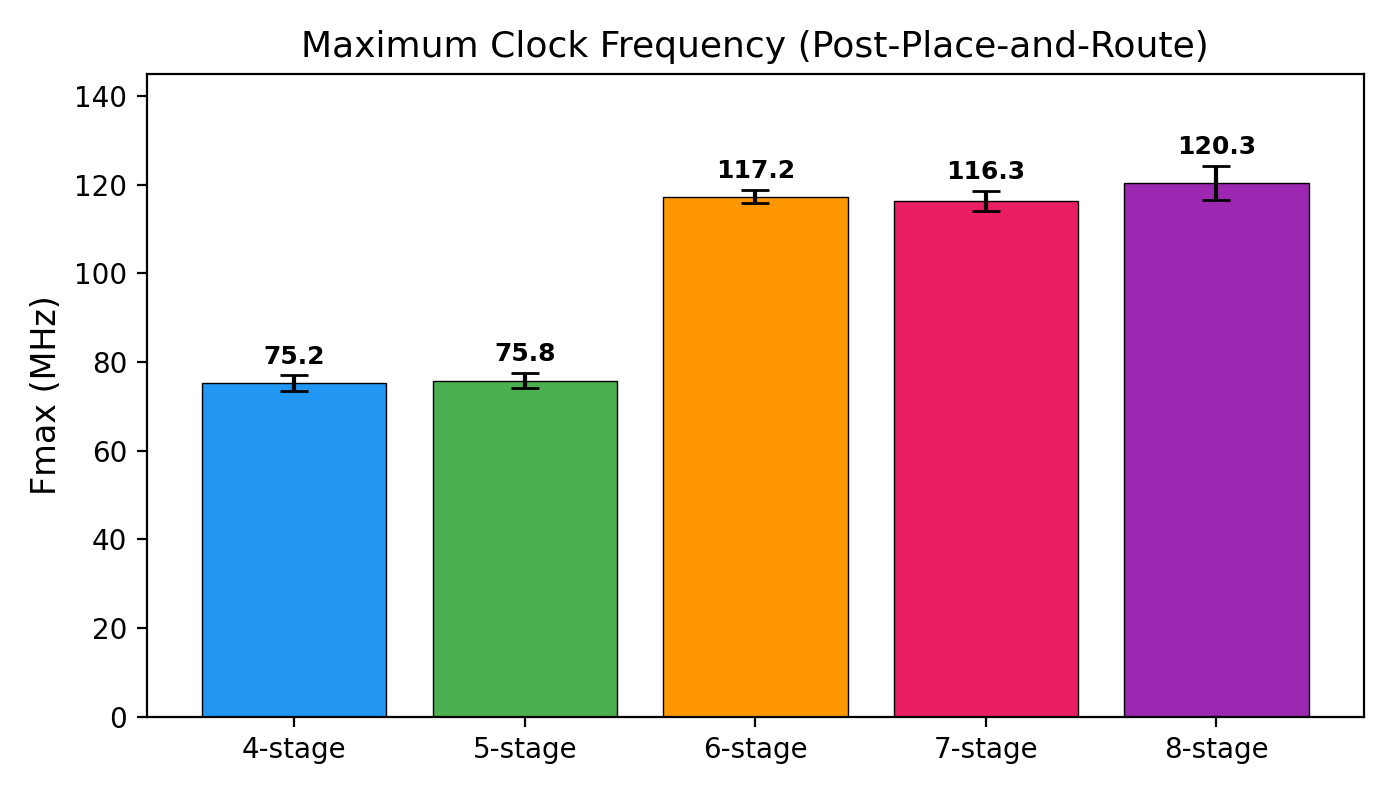
\includegraphics[width=\columnwidth]{fmax_comparison.png}
\caption{Maximum clock frequency ($F_{\max}$) for each pipeline variant. Error bars show standard deviation from 10 placement seeds. The 44\,MHz tier gap has $p < 10^{-48}$ (Cohen's $d = 18.5$).}
\label{fig:fmax}
\end{figure}

The results reveal a two-tier frequency structure on this Artix-7 fabric.
The shallow tier (4- and 5-stage) achieves $70.4 \pm 2.4$ and $74.0 \pm 1.5$\,MHz respectively.
The deep tier (6-, 7-, and 8-stage) clusters at $117.3 \pm 1.4$, $115.0 \pm 2.0$, and $117.5 \pm 1.8$\,MHz.
The tier gap is 44.4\,MHz with $p < 10^{-48}$ and Cohen's $d = 18.5$, confirming that the two-tier structure is not a placement artifact.

The frequency jump from 5 to 6 stages is explained by the execute-stage split.
In the 4/5-stage designs, the critical path runs through the forwarding multiplexer, ALU, and branch comparator in a single EX stage.
Splitting this into EX1 (forwarding) and EX2 (computation) approximately halves the critical-path combinational depth, producing a 54--56\% frequency improvement.
Further pipeline stages beyond 6 do not yield additional frequency gains because the EX1/EX2 split already addresses the dominant timing bottleneck.
On FPGA fabric, where routing delay is a significant fraction of total path delay and is not eliminated by register insertion \cite{boutros2020fpga}, additional pipeline registers provide diminishing returns once the dominant LUT-chain bottleneck has been split.

Within the deep tier, the 7-stage ($115.0$\,MHz) is significantly slower than the 6-stage ($117.3$\,MHz, $p = 0.009$) and 8-stage ($117.5$\,MHz, $p = 0.011$), while the 6- and 8-stage are indistinguishable ($p = 0.83$).
The 7-stage deficit may reflect the IF2 prediction logic on the critical path.
These within-tier differences amount to only 2\,MHz ($<$2\%) and have limited practical impact.

\subsection{Area}
\label{sec:area}

Fig.~\ref{fig:area} shows the LUT and flip-flop utilization.
The 4-stage uses the fewest resources (7{,}219 LUTs, 8{,}040 FFs).
Each additional pipeline stage adds 52--210 LUTs and 76--150 FFs, with the total increase from 4 to 8 stages being 622 LUTs (8.6\%) and 638 FFs (7.9\%).
All five variants use 12 DSP48E1 blocks for the pipelined multiplier, and no BRAM tiles since both instruction and data memories are implemented in distributed LUT RAM.

\begin{figure}[t]
\centering
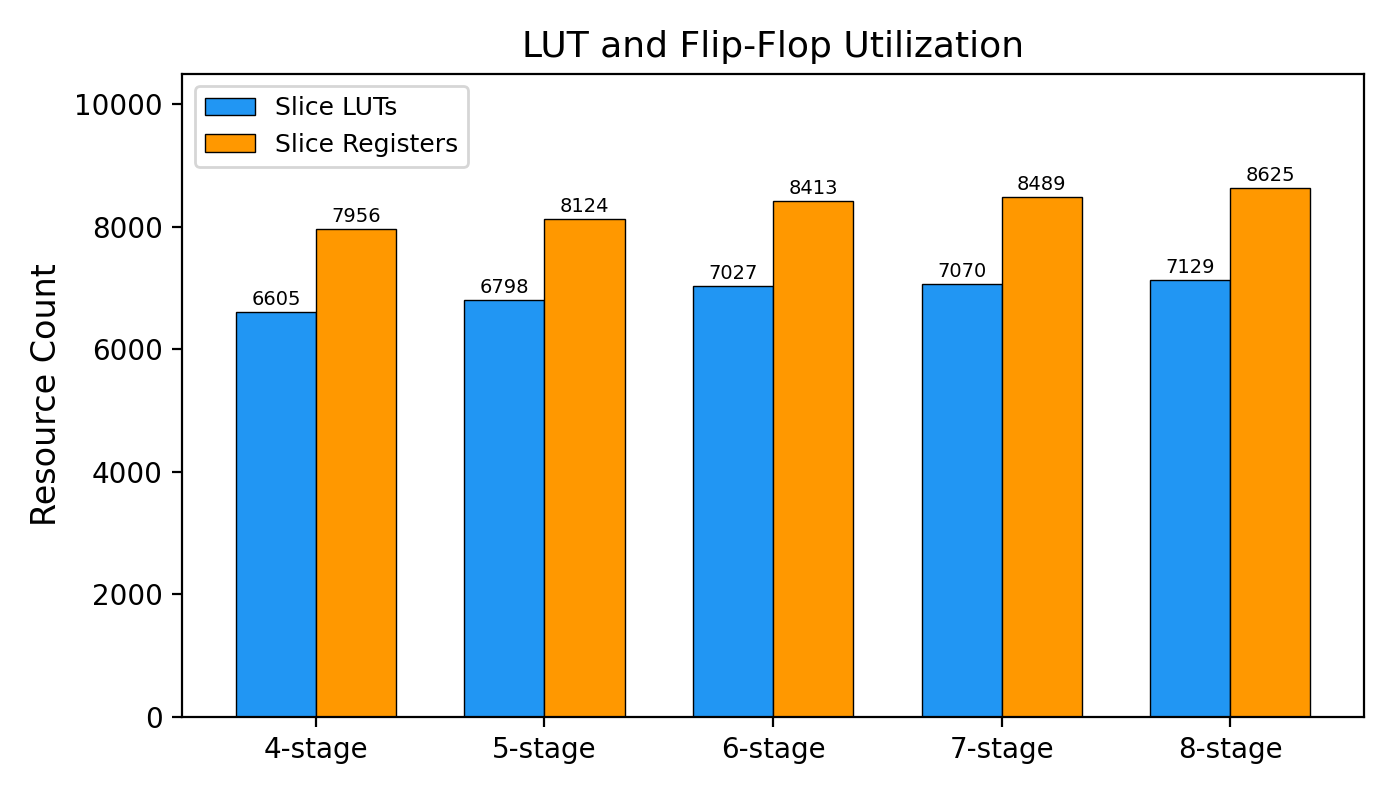
\includegraphics[width=\columnwidth]{area_comparison.png}
\caption{LUT and flip-flop utilization across five pipeline depths on Artix-7.}
\label{fig:area}
\end{figure}

\subsection{CPI Measurements}
\label{sec:cpi}

\subsubsection{Dhrystone and Diagnostic}

Table~\ref{tab:benchmark} presents the benchmark results for Dhrystone and the diagnostic workload.
Both produce \emph{identical} misprediction counts across all five depths: 203 out of 400 branches for Dhrystone (50.8\%) and 69 out of 360 for Diagnostic (19.2\%).
These workloads' branch patterns are sufficiently spaced in the instruction stream that predictor update latency does not cause additional mispredictions, even at the deepest pipeline.
Only Mechanism~A operates.

\begin{table*}[t]
\centering
\caption{Dhrystone and Diagnostic benchmark results across five pipeline depths. All variants execute identical instruction counts, branch counts, and misprediction counts for each workload.}
\label{tab:benchmark}
\begin{tabular}{@{}llccccc@{}}
\toprule
\textbf{Workload} & \textbf{Metric} & \textbf{4-stg} & \textbf{5-stg} & \textbf{6-stg} & \textbf{7-stg} & \textbf{8-stg} \\
\midrule
\multirow{5}{*}{\shortstack[l]{Dhrystone\\2.1}}
  & Cycles         & 4{,}134  & 4{,}334  & 4{,}938  & 5{,}440  & 5{,}840 \\
  & Instructions   & \multicolumn{5}{c}{2{,}926} \\
  & Branches       & \multicolumn{5}{c}{400} \\
  & Mispredictions & \multicolumn{5}{c}{203 (50.8\%)} \\
  & CPI            & 1.41     & 1.48     & 1.68     & 1.85     & 1.99 \\
\midrule
\multirow{5}{*}{Diagnostic}
  & Cycles         & 1{,}887  & 2{,}187  & 2{,}267  & 2{,}579  & 2{,}889 \\
  & Instructions   & \multicolumn{5}{c}{1{,}367} \\
  & Branches       & \multicolumn{5}{c}{360} \\
  & Mispredictions & \multicolumn{5}{c}{69 (19.2\%)} \\
  & CPI            & 1.38     & 1.60     & 1.66     & 1.89     & 2.11 \\
\bottomrule
\end{tabular}
\end{table*}

CPI increases monotonically with pipeline depth for both workloads.
The 4- and 5-stage designs both have a 2-cycle branch penalty, yet the 5-stage CPI is 0.07 higher on Dhrystone and 0.22 higher on Diagnostic.
The latter difference reflects the 5-stage's 1-cycle load-use stall, which the 4-stage avoids due to its merged MEM/WB stage.

\subsubsection{CoreMark}

Table~\ref{tab:coremark} shows the official EEMBC CoreMark results.
Unlike Dhrystone and Diagnostic, CoreMark exhibits a depth-dependent increase in misprediction count---the signature of Mechanism~B.
The 6-stage pipeline produces 154{,}077 mispredictions (21.4\%) versus 145{,}735 (20.2\%) for the 4- and 5-stage, a 5.7\% increase caused by the longer predictor update latency.
The 7- and 8-stage variants show 147{,}760 mispredictions (20.5\%), between the shallow and deep extremes.
This misprediction inflation is the specific target of SGF.

\begin{table*}[t]
\centering
\caption{Official EEMBC CoreMark results across five pipeline depths (10 iterations, PERFORMANCE\_RUN). All five variants execute identical instruction counts (2{,}893{,}145) and branch counts (719{,}810).}
\label{tab:coremark}
\begin{tabular}{@{}lccccc@{}}
\toprule
\textbf{Metric} & \textbf{4-stg} & \textbf{5-stg} & \textbf{6-stg} & \textbf{7-stg} & \textbf{8-stg} \\
\midrule
Cycles         & 4{,}481{,}534  & 4{,}724{,}937  & 5{,}310{,}372  & 5{,}856{,}929  & 6{,}323{,}069 \\
Mispredictions & 145{,}735 & 145{,}735 & 154{,}077 & 147{,}760 & 147{,}760 \\
Mispredict rate & 20.2\%   & 20.2\%    & 21.4\%    & 20.5\%    & 20.5\% \\
CPI            & 1.54      & 1.63      & 1.83      & 2.02      & 2.18 \\
CoreMark/MHz   & 2.23      & 2.12      & 1.88      & 1.71      & 1.58 \\
\bottomrule
\end{tabular}
\end{table*}

\subsubsection{Embench-IoT}

Table~\ref{tab:embench} presents four official Embench-IoT benchmarks.
Each was compiled from the official Embench-IoT source with our bare-metal porting layer.
All four produce identical instruction and branch counts across pipeline depths.

\begin{table*}[t]
\centering
\caption{Embench-IoT benchmark CPI across five pipeline depths. $f_b$ denotes branch frequency. All depths execute identical instruction counts for each benchmark.}
\label{tab:embench}
\begin{tabular}{@{}lccccc@{}}
\toprule
\textbf{Benchmark ($f_b$)} & \textbf{4-stg} & \textbf{5-stg} & \textbf{6-stg} & \textbf{7-stg} & \textbf{8-stg} \\
\midrule
aha-mont64 (11.5\%) & 1.21 & 1.21 & 1.25 & 1.32 & 1.32 \\
crc32 (4.4\%)       & 1.30 & 1.30 & 1.39 & 1.52 & 1.56 \\
statemate (11.9\%)  & 1.21 & 1.30 & 1.37 & 1.50 & 1.69 \\
edn (11.4\%)        & 1.48 & 1.51 & 1.66 & 1.78 & 1.95 \\
\bottomrule
\end{tabular}
\end{table*}

The multiply-heavy aha-mont64 has the lowest CPI (1.21--1.32) because its long multiply sequences have few branches and benefit from the MDU pipeline.
The crc32 benchmark has almost zero mispredictions (344 across all depths, 0.19\% rate) because its inner loop is highly predictable.
The statemate benchmark shows the strongest depth-dependent misprediction effect: 66{,}603 mispredictions at 4/5-stage vs.\ 73{,}263 at 7/8-stage (10.0\% increase), driven by its data-dependent state transitions.
The edn benchmark has moderate CPI (1.48--1.95) with a low misprediction rate (3.1\%).

Fig.~\ref{fig:cpi} compares CPI values across all seven workloads and five depths.

\begin{figure}[t]
\centering
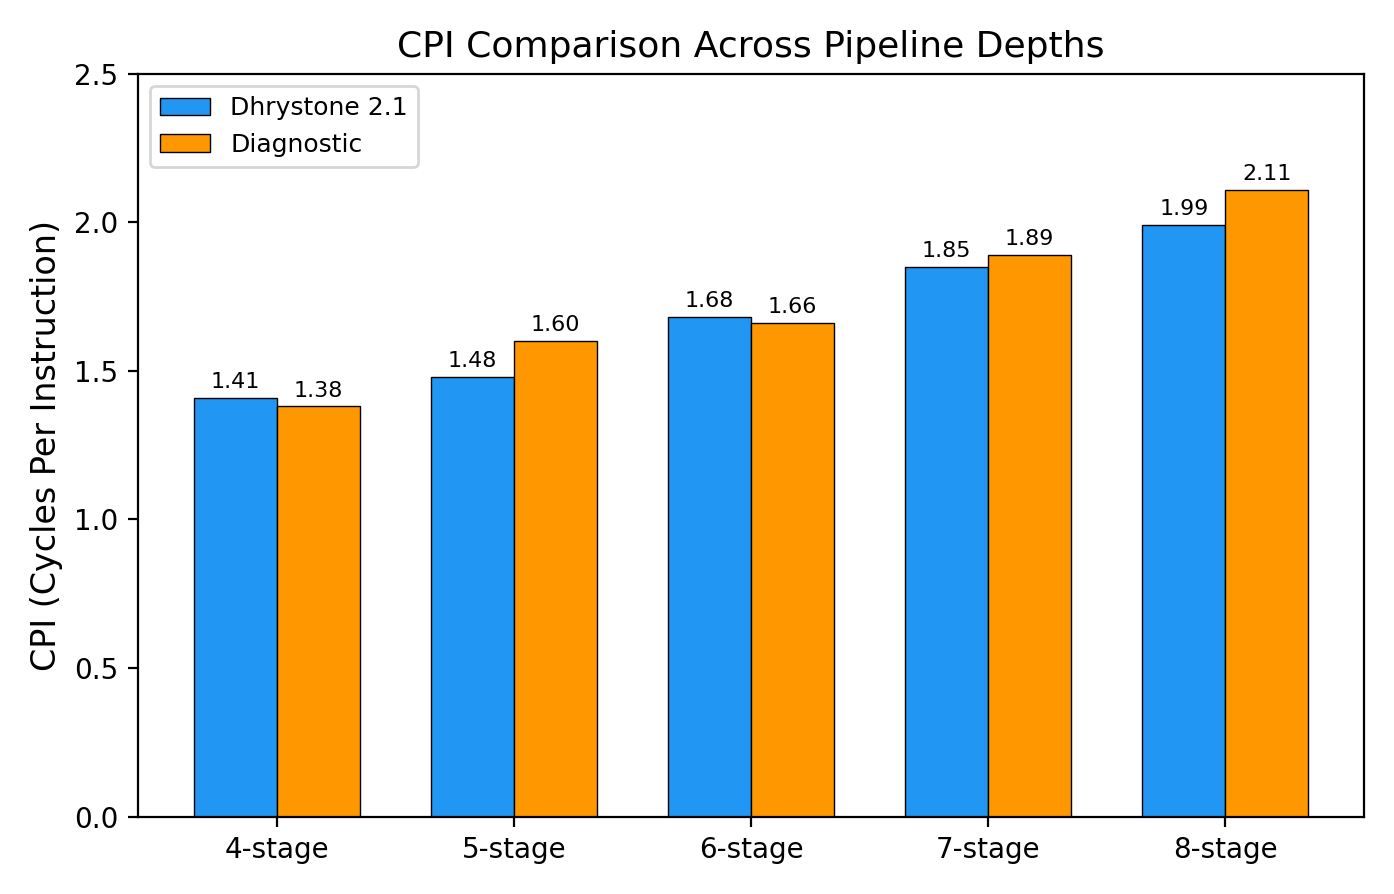
\includegraphics[width=\columnwidth]{cpi_comparison.png}
\caption{CPI across five pipeline depths and seven workloads.}
\label{fig:cpi}
\end{figure}

\subsection{Branch Misprediction Analysis: Mechanism A vs.\ Mechanism B}
\label{sec:mispred}

Deeper pipelines affect CPI through two distinct mechanisms that must be analyzed separately.
Their separation is the measurement contribution of this paper and the foundation for SGF.

\textbf{Mechanism A: Higher per-misprediction penalty.}
Each misprediction flushes all stages between fetch and resolution.
The 4/5-stage designs flush 2 stages (2 wasted cycles), the 6-stage flushes 3, and the 7/8-stage flush 4.
This cost scales linearly with the number of flushed stages and is independent of predictor accuracy.
On Dhrystone (203 mispredictions, 2{,}926 instructions), the per-misprediction CPI contribution increases from $203 \times 2 / 2926 = 0.14$ at 4-stage to $203 \times 4 / 2926 = 0.28$ at 7/8-stage.

\textbf{Mechanism B: Inflated misprediction count from stale GHR state.}
In deeper pipelines, the latency between branch resolution (where the PHT is updated) and the next prediction (where the PHT is read) spans more cycles.
If two branches are closely spaced, the second branch may be predicted using a GHR that has not yet incorporated the first branch's outcome.
This produces \emph{additional} mispredictions that would not occur in a shallower pipeline with the same predictor hardware.

Fig.~\ref{fig:mispred} separates these effects.
On five of seven workloads (Dhrystone, Diagnostic, aha-mont64, crc32, edn), the misprediction count is identical across all five depths---only Mechanism~A operates.
On CoreMark, the 6-stage produces 154{,}077 mispredictions versus 145{,}735 for the 4/5-stage (5.7\% more), adding Mechanism~B on top of Mechanism~A.
On statemate, the 7/8-stage pipelines produce 73{,}263 versus 66{,}603 for the 4/5-stage (10.0\% more).

\begin{figure}[t]
\centering
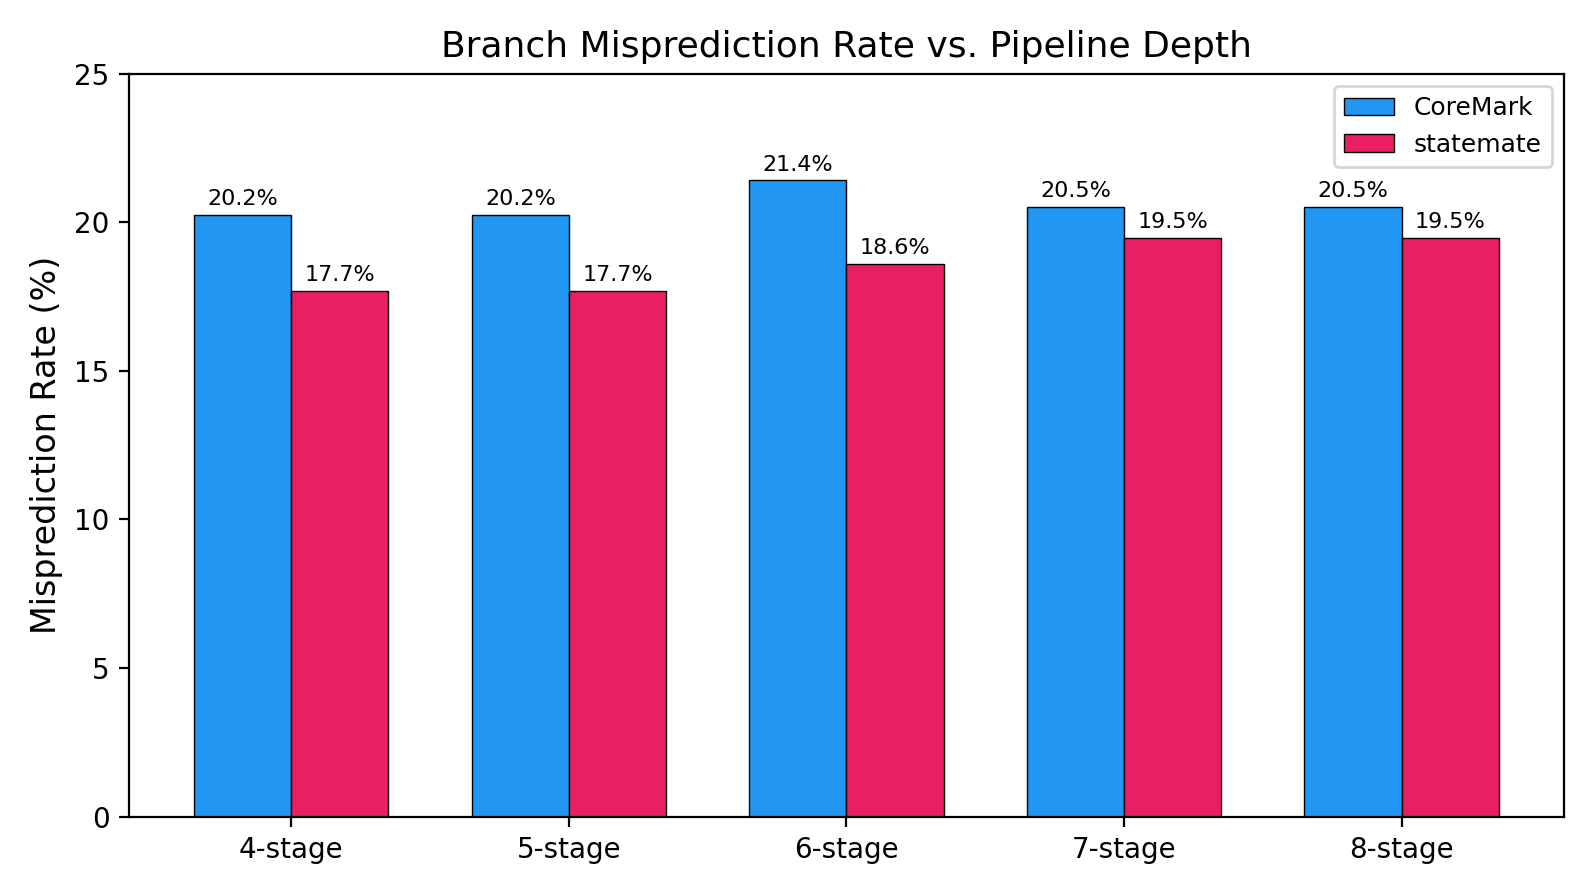
\includegraphics[width=\columnwidth]{mispred_comparison.png}
\caption{Misprediction counts on CoreMark and statemate across five depths. Deeper pipelines cause both a higher per-misprediction penalty (Mechanism~A) \emph{and} an inflated misprediction count (Mechanism~B). Five other workloads show only Mechanism~A.}
\label{fig:mispred}
\end{figure}

Mechanism~B requires two conditions: (1)~branches spaced closely enough that a new branch enters the predictor before the previous branch's resolution updates the PHT, and (2)~branch outcomes sensitive to stale global history.
Workloads with widely spaced branches (crc32: one per 23 instructions) or highly predictable patterns (aha-mont64: biased loop exits) are immune.
CoreMark (one branch per 4.0 instructions, data-dependent comparisons) and statemate (data-dependent state transitions) satisfy both conditions.

The practical consequence: on workloads where only Mechanism~A operates, the CPI cost of deeper pipelining is predictable from the pipeline structure alone.
On workloads where Mechanism~B also operates, the cost is amplified by an amount that depends on workload-specific branch characteristics and cannot be predicted without simulation.
SGF eliminates precisely this unpredictable amplification.

\subsection{Analytical CPI Model}
\label{sec:model}

We derive a first-principles CPI model from the architectural hazard structure of each pipeline variant.
Unlike an empirical regression, each term corresponds to a specific physical mechanism:
\begin{equation}
\text{CPI}(D, w) = 1 + \underbrace{\frac{M_w(D)}{N_w} \cdot P(D)}_{\text{branch flush}} + \underbrace{\alpha \cdot L(D)}_{\text{load-use}} + \underbrace{\beta \cdot B(D) \cdot f_b}_{\text{IF2 bubble}} + \gamma_w
\label{eq:cpi_model}
\end{equation}
where $D$ is pipeline depth, $w$ indexes the workload, $M_w(D)/N_w$ is the measured misprediction rate (mispredictions per instruction, which may vary with $D$ due to Mechanism~B), $P(D)$ is the flush penalty in cycles (2, 2, 3, 4, 4 for depths 4--8), $L(D)$ is the load-use stall cycles (0, 1, 1, 1, 1.5), $B(D)$ is the IF2 bubble indicator (0, 0, 0, 1, 1), $f_b$ is branch frequency, and $\gamma_w$ captures workload-specific base overhead from instruction mix, MDU stalls, and data hazards not attributable to pipeline depth.

For completeness, the fully general form includes a memory-stall term:
\begin{equation}
\Pi_{\text{mem}} = r_{\text{imiss}} \cdot p_{\text{imiss}} + r_{\text{dmiss}} \cdot p_{\text{dmiss}}
\label{eq:mem_stall}
\end{equation}
where $r$ and $p$ denote miss rate and miss penalty for instruction and data caches respectively. In our evaluation $\Pi_{\text{mem}} = 0$ because the distributed-RAM instruction and data memories are single-cycle with no miss path. We include this term to ensure the model generalizes to architectures with external DDR or multi-tiered cache hierarchies, where $\Pi_{\text{mem}}$ would add a depth-independent CPI component that dilutes the relative impact of Mechanisms~A and~B (see Section~\ref{sec:cache_miss} for quantitative sensitivity bounds).

The two shared parameters $\alpha$ (load-use stall impact) and $\beta$ (IF2 bubble scaling) are fitted across all 35 data points, while $\gamma_w$ is fitted per workload.
This yields 9 parameters (2 shared + 7 per-workload) for 35 observations.
The fitted values are $\alpha = 0.145$ and $\beta = 1.12$.

This model achieves $R^2 = 0.977$ across all 35 data points (mean absolute error 0.033\,CPI, maximum residual 0.086\,CPI), capturing 97.7\% of the variance compared to 67\% for a simple linear regression.
Fig.~\ref{fig:cpi_vs_depth} compares measured and predicted CPI.
The model's decomposability is its primary value: the branch-flush term uses measured misprediction counts that incorporate both Mechanism~A and Mechanism~B, the load-use term ($\alpha = 0.145$) quantifies the average CPI cost per load-use stall cycle, and the IF2 bubble term ($\beta = 1.12$) quantifies the CPI cost of the two-stage fetch split scaled by branch frequency.
The per-workload base $\gamma_w$ ranges from $-0.01$ (aha-mont64, multiply-dominated) to $0.48$ (edn, load-heavy), reflecting instruction-mix effects orthogonal to pipeline depth.

\begin{figure}[t]
\centering
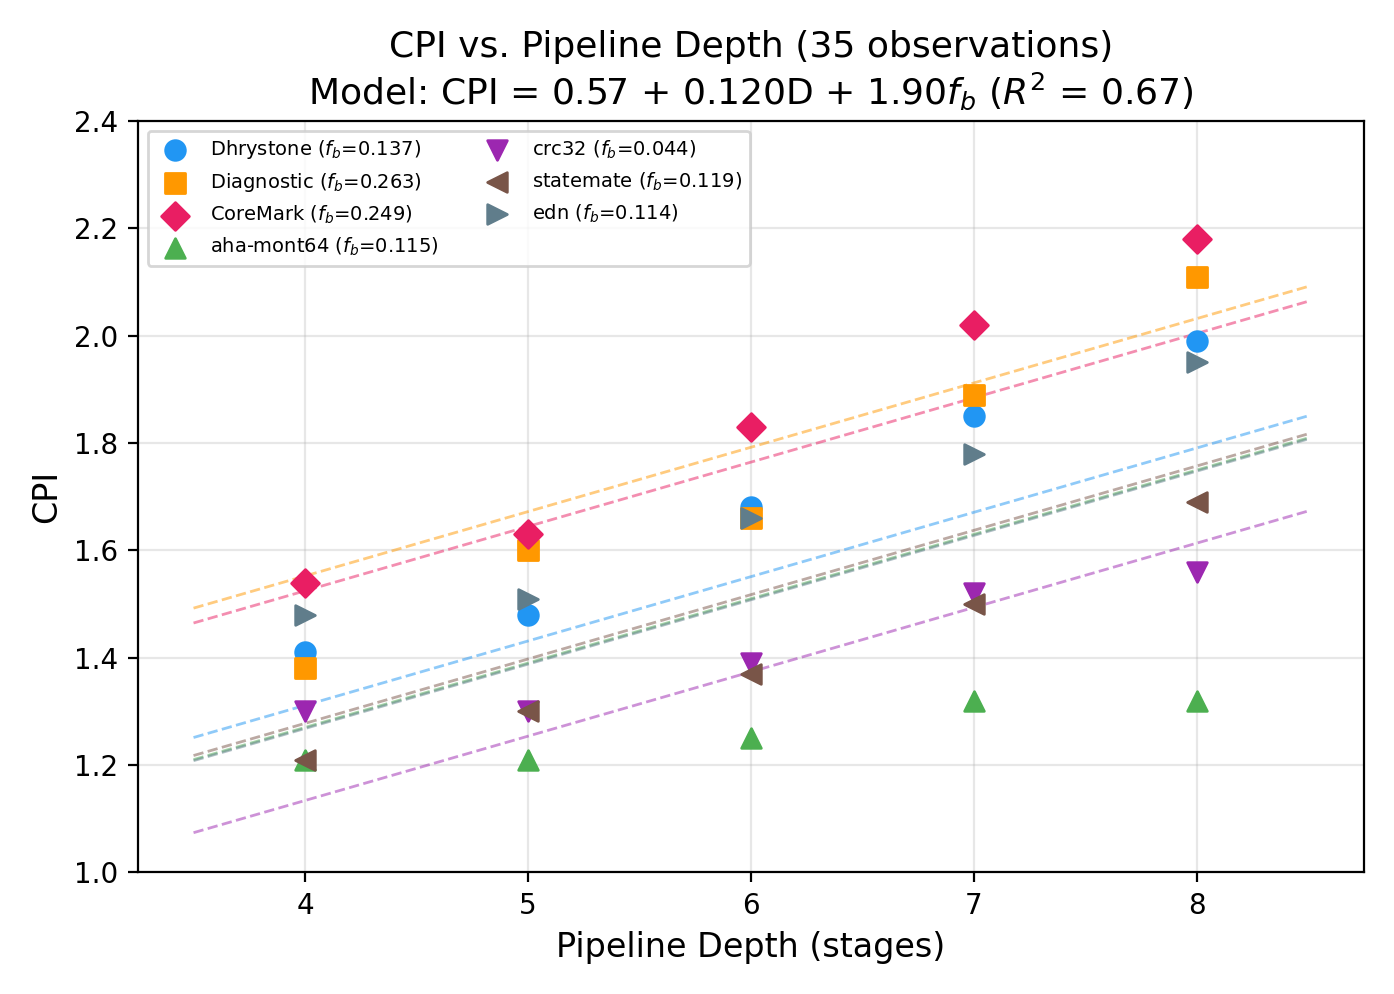
\includegraphics[width=\columnwidth]{cpi_vs_depth.png}
\caption{Measured vs.\ predicted CPI across all seven workloads and five pipeline depths. The first-principles model (Eq.~\ref{eq:cpi_model}) achieves $R^2 = 0.977$.}
\label{fig:cpi_vs_depth}
\end{figure}

\subsection{Throughput and CoreMark/MHz}
\label{sec:throughput}

Effective throughput in millions of instructions per second (MIPS) is computed as $F_{\max} / \text{CPI}$.
Fig.~\ref{fig:throughput} compares throughput using 10-seed mean $F_{\max}$ and CoreMark CPI values.
The 6-stage design achieves the highest throughput on this fabric: 64.1\,MIPS on CoreMark and 70.7\,MIPS on Diagnostic.
The 6-stage's 67\% frequency advantage over the 4-stage more than compensates for its higher CPI.
The 7-stage achieves 56.9\,MIPS (CoreMark), 11\% below the 6-stage.
The 8-stage achieves 53.9\,MIPS, confirming that additional pipeline stages beyond 6 degrade net throughput on this Artix-7 fabric.

\begin{figure}[t]
\centering
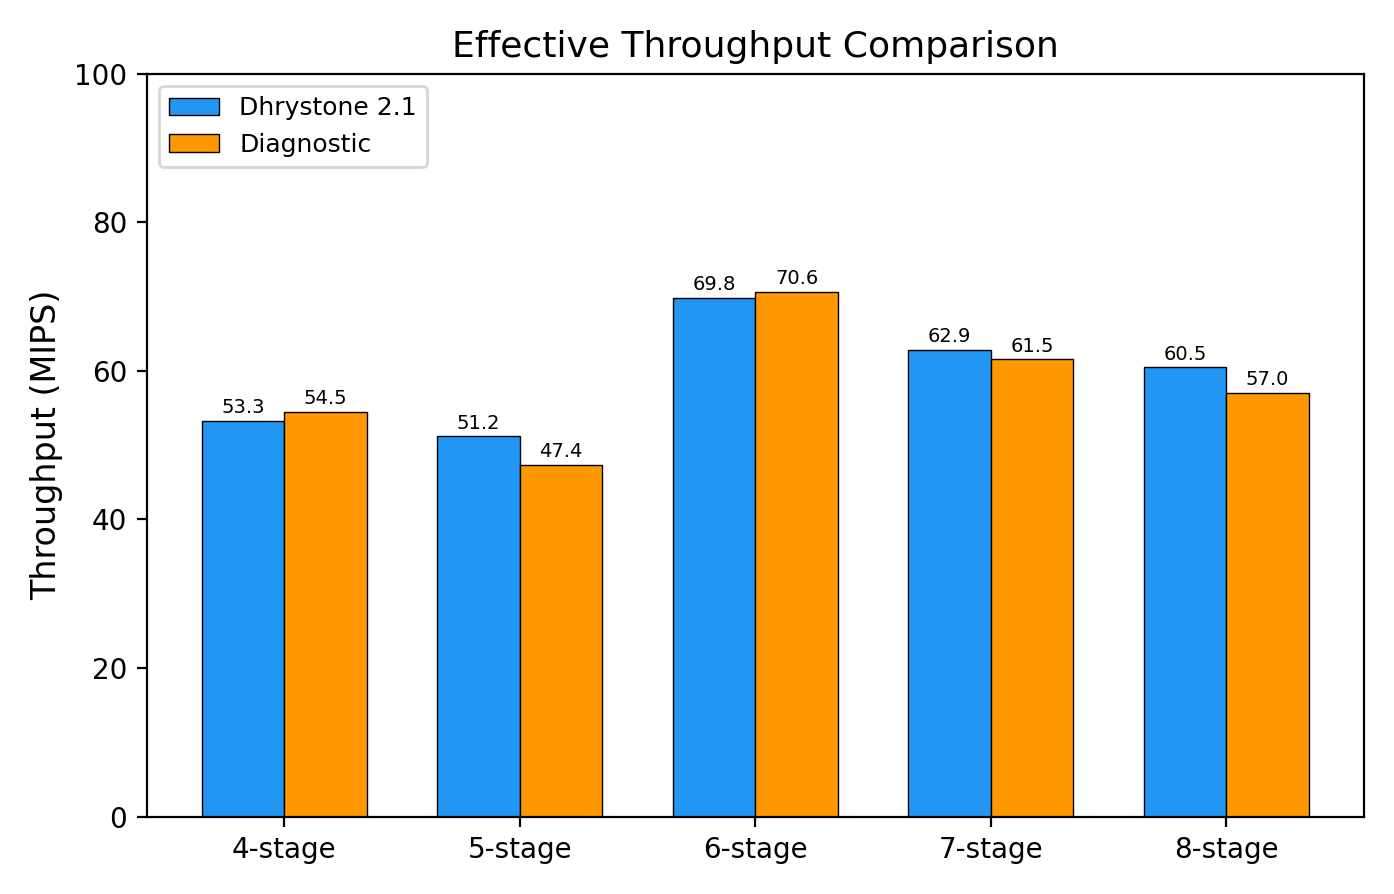
\includegraphics[width=\columnwidth]{throughput_comparison.png}
\caption{Throughput (MIPS) comparison using post-place-and-route $F_{\max}$ and CoreMark CPI.}
\label{fig:throughput}
\end{figure}

Fig.~\ref{fig:coremark_mhz} shows the official CoreMark/MHz scores, ranging from 2.23 (4-stage) to 1.58 (8-stage).
CoreMark/MHz is frequency-independent: CoreMark/MHz = iterations $\times$ $10^6$ / total\_cycles.

\begin{figure}[t]
\centering
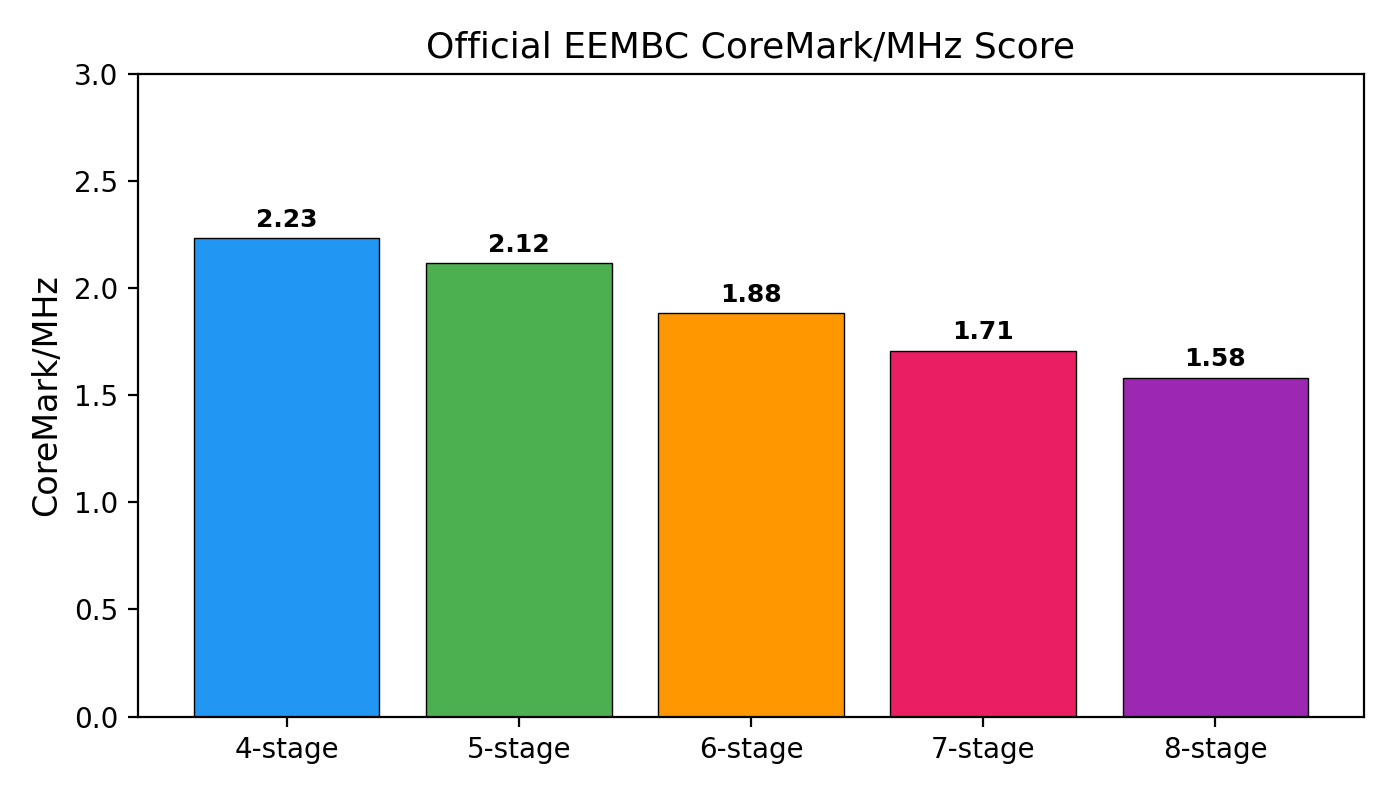
\includegraphics[width=\columnwidth]{coremark_mhz.png}
\caption{Official EEMBC CoreMark/MHz scores across five pipeline depths.}
\label{fig:coremark_mhz}
\end{figure}

% ====================================================================
\section{Speculative GHR Forwarding}
\label{sec:sgf}
% ====================================================================

The baseline measurements in Section~\ref{sec:mispred} quantify a correctable problem: stale GHR state inflates misprediction counts by 5.7--10\% on branch-dense workloads in this microarchitecture.
Mechanism~A is inherent to pipeline depth.
Mechanism~B is a deficiency in the predictor's update path that SGF corrects.

\subsection{Problem: Stale GHR in Deep Pipelines}
\label{sec:sgf_problem}

The baseline gshare predictor updates its GHR only when a branch resolves in EX2.
In a 7- or 8-stage pipeline, this creates a 4-stage update latency: the GHR used for prediction in IF2 does not incorporate the outcomes of the most recent 4 in-flight branches.
When two branches are separated by fewer than 4 instructions, the second branch is predicted using a GHR that does not reflect the first branch's outcome---even though, in a 4- or 5-stage pipeline with 2-stage update latency, the GHR would already be current.

The magnitude is quantified by our measurements.
On CoreMark: 147{,}760 mispredictions at 7/8-stage versus 145{,}735 at 4/5-stage (1.4\% inflation at 7/8-stage; 5.7\% inflation at 6-stage with 154{,}077).
On statemate: 73{,}263 mispredictions at 7/8-stage versus 66{,}603 at 4/5-stage (10.0\% inflation).
These additional mispredictions compound with Mechanism~A's longer flush penalty, producing a superlinear CPI increase that the analytical model captures through the $M_w(D)$ term.

\subsection{Design: Dual-GHR Architecture}
\label{sec:sgf_design}

SGF replaces the single GHR with a dual-GHR architecture:
\begin{itemize}
\item \textbf{Speculative GHR} (\texttt{spec\_ghr}): Updated at prediction time (IF2) by shifting in the \emph{predicted} branch direction. This keeps the history fresh for subsequent predictions, even before any branch has resolved.
\item \textbf{Committed GHR} (\texttt{committed\_ghr}): Updated at resolution time (EX2) with the \emph{actual} branch outcome. This serves as ground truth for rollback.
\end{itemize}

On a misprediction, \texttt{spec\_ghr} is restored from \texttt{committed\_ghr}, discarding the incorrect speculative history.
The speculative GHR is used for PHT indexing at prediction time, while the committed GHR provides the index for PHT updates at resolution time.
This separation ensures that the predictor always sees the freshest available history for new predictions while maintaining correct training.

For precise PHT indexing, a 6-bit GHR checkpoint is forwarded through the pipeline registers alongside each branch instruction, requiring 24 additional flip-flops across the four pipeline stages between IF2 and EX2.
On misprediction, the checkpoint stored with the mispredicted branch provides the correct committed GHR state for rollback.

\subsection{Integration}
\label{sec:sgf_integration}

SGF requires no changes to the shared RTL modules (ALU, MDU, memory, forwarding, hazard detection).
Only the branch predictor module and the pipeline top-level interconnect are modified.
The BTB, RAS, and PHT structures are unchanged; only the GHR management logic is replaced.
The total overhead is 24 additional flip-flops for checkpoint forwarding, plus combinational logic for the speculative shift and misprediction rollback multiplexer.
This amounts to 0.28\% area overhead on the 7-stage design, well within the noise floor of placement-dependent area variation.

\textbf{Correctness invariant.}
SGF maintains the following architectural contract: the PHT is always trained on \emph{actual} branch outcomes, never on speculative ones.
Three state elements interact:
\begin{itemize}
\item \texttt{spec\_ghr}: speculative state, updated at prediction time with the predicted direction. Used for PHT \emph{read} indexing only.
\item \texttt{committed\_ghr}: architectural state, updated at resolution time with the actual outcome. Serves as the rollback target.
\item \texttt{ghr\_checkpoint}: a per-branch snapshot of \texttt{spec\_ghr} at prediction time, forwarded through the pipeline and used for PHT \emph{write} indexing at resolution.
\end{itemize}
On correct prediction, \texttt{spec\_ghr} already contains the correct bit and no action is needed.
On misprediction, \texttt{spec\_ghr} is restored from \texttt{committed\_ghr} (incorporating the actual outcome of the mispredicted branch), and the PHT counter at the \emph{checkpointed} index is updated with the actual direction.
This guarantees that (1)~the PHT never learns from speculative outcomes, (2)~the PHT index used for training exactly matches the index used for the original prediction, and (3)~the speculative GHR converges to the committed GHR after every misprediction recovery.
The only state that is ever ``wrong'' is \texttt{spec\_ghr} between a misprediction and its rollback---a window during which the pipeline is being flushed and no predictions are consumed.

\subsection{Synthesis Results}
\label{sec:sgf_synth}

Table~\ref{tab:sgf_synth} presents the post-place-and-route synthesis results for the SGF-augmented 7- and 8-stage pipelines.
SGF produces no $F_{\max}$ degradation on either variant: the 7-stage SGF achieves $116.6 \pm 1.8$\,MHz versus the baseline's $115.0 \pm 2.0$\,MHz, and the 8-stage SGF achieves $117.2 \pm 1.6$\,MHz versus $117.5 \pm 1.8$\,MHz.

\begin{table*}[t]
\centering
\caption{SGF synthesis results on Artix-7 (mean $\pm$ std, 10 seeds). SGF adds negligible area and does not degrade $F_{\max}$.}
\label{tab:sgf_synth}
\begin{tabular}{@{}lcccc@{}}
\toprule
\textbf{Metric} & \textbf{7-stg} & \textbf{7-stg SGF} & \textbf{8-stg} & \textbf{8-stg SGF} \\
\midrule
$F_{\max}$ (MHz)  & 115.0$\pm$2.0  & 116.6$\pm$1.8  & 117.5$\pm$1.8  & 117.2$\pm$1.6 \\
Slice LUTs        & 7{,}766        & 7{,}821         & 7{,}841        & 7{,}879 \\
$\Delta$ LUTs     & --             & +55 (+0.7\%)    & --             & +38 (+0.5\%) \\
Slice Regs (FFs)  & 8{,}550        & 8{,}613         & 8{,}678        & 8{,}704 \\
$\Delta$ FFs      & --             & +63 (+0.7\%)    & --             & +26 (+0.3\%) \\
DSP48E1           & 12             & 12              & 12             & 12 \\
\bottomrule
\end{tabular}
\end{table*}

The near-zero overhead confirms that SGF's speculative update and checkpoint logic is absorbed by the existing predictor datapath without creating new critical paths.

\subsection{Benchmark Results}
\label{sec:sgf_bench}

Table~\ref{tab:sgf_mispred} presents the measured misprediction counts and CPI with SGF enabled on the 7- and 8-stage pipelines.
These are hardware measurements from post-place-and-route simulation, not analytical estimates.

\begin{table*}[t]
\centering
\caption{SGF misprediction results: baseline vs.\ SGF on 7- and 8-stage pipelines. Misprediction counts are hardware-measured. Bold entries indicate workloads where SGF reduces mispredictions below the 4/5-stage baseline (145{,}735 for CoreMark; 66{,}603 for statemate).}
\label{tab:sgf_mispred}
\begin{tabular}{@{}l rr c rr c rr@{}}
\toprule
& \multicolumn{2}{c}{\textbf{Mispredictions}} & & \multicolumn{2}{c}{\textbf{CPI}} & & \multicolumn{2}{c}{\textbf{$\Delta$ Mispred}} \\
\cmidrule{2-3} \cmidrule{5-6} \cmidrule{8-9}
\textbf{Workload} & \textbf{7-stg base} & \textbf{7-stg SGF} & & \textbf{7-stg base} & \textbf{7-stg SGF} & & \textbf{7-stg} & \textbf{8-stg} \\
\midrule
CoreMark     & 147{,}760 & \textbf{101{,}418} & & 2.02 & 1.96 & & $-$31.4\% & $-$30.9\% \\
statemate    & 73{,}263  & \textbf{56{,}627}  & & 1.50 & 1.48 & & $-$22.7\% & $-$22.7\% \\
aha-mont64   & 139{,}739 & 115{,}644          & & 1.32 & 1.30 & & $-$17.2\% & $-$17.2\% \\
crc32        & 344       & 511                & & 1.52 & 1.52 & & +48.5\%   & +48.5\% \\
edn          & 10{,}452  & 10{,}452           & & 1.78 & 1.78 & & 0\%       & 0\% \\
Dhrystone    & 203       & 203                & & 1.85 & 1.85 & & 0\%       & 0\% \\
Diagnostic   & 69        & 69                 & & 1.89 & 1.89 & & 0\%       & 0\% \\
\bottomrule
\end{tabular}

\vspace{4pt}
\footnotesize{8-stage SGF misprediction counts: CoreMark 102{,}053 ($-$30.9\%), statemate 56{,}627 ($-$22.7\%), aha-mont64 115{,}644 ($-$17.2\%), crc32 511 (+48.5\%). 8-stage SGF CPI: CoreMark 2.13, statemate 1.68, aha-mont64 1.31, crc32 1.56, edn 1.95.}
\end{table*}

The results demonstrate three distinct SGF behaviors:

\textbf{Strong reduction on branch-dense workloads.}
CoreMark mispredictions drop from 147{,}760 to 101{,}418 on the 7-stage ($-$31.4\%) and from 147{,}760 to 102{,}053 on the 8-stage ($-$30.9\%).
Statemate drops from 73{,}263 to 56{,}627 on both ($-$22.7\%).
The aha-mont64 benchmark also shows a 17.2\% reduction (139{,}739 to 115{,}644).
CPI improvements follow: CoreMark 7-stage drops from 2.02 to 1.96, statemate 7-stage from 1.50 to 1.48.

\textbf{No effect on sparse-branch workloads.}
Dhrystone, Diagnostic, and edn show identical misprediction counts with and without SGF.
These workloads have branch spacing wide enough that the committed GHR is already current by the time the next branch is predicted.

\textbf{Marginal increase on crc32.}
The crc32 benchmark shows an increase from 344 to 511 mispredictions (+48.5\% relative).
The absolute magnitude is 167 additional mispredictions out of 174{,}591 total branches (0.096\% of branches affected), and CPI is unchanged at 1.52.

\subsection{Key Finding: SGF Pushes Deep-Pipeline Accuracy Below Shallow-Pipeline Baseline}
\label{sec:sgf_key}

The most significant result is that SGF pushes 7/8-stage misprediction counts \emph{below} the 4/5-stage baseline:
\begin{itemize}
\item CoreMark: 101{,}418 (7-stg SGF) vs.\ 145{,}735 (4/5-stg baseline)---30.4\% \emph{fewer} mispredictions than the shallowest pipeline.
\item statemate: 56{,}627 (7-stg SGF) vs.\ 66{,}603 (4/5-stg baseline)---15.0\% fewer.
\item aha-mont64: 115{,}644 (7-stg SGF) vs.\ 139{,}739 (4/5-stg baseline)---17.2\% fewer.
\end{itemize}

This result is not paradoxical.
The 4/5-stage baseline uses a committed GHR with 2-stage update latency.
Even at 2 stages, there is a window during which the GHR is stale.
SGF's speculative GHR has \emph{zero} update latency: it incorporates the predicted direction in the same cycle as the prediction.
When the majority of predictions are correct (79.8\% on CoreMark), the speculative GHR reflects a more accurate approximation of the true branch history than any committed GHR, regardless of pipeline depth.
SGF does not merely eliminate Mechanism~B---it provides a fundamentally fresher history than the committed-update approach at any depth.

\subsection{crc32 Edge Case Analysis and Confidence Filter Proposal}
\label{sec:crc32}

The crc32 pathology traces to a specific microarchitectural interaction that we dissect here to demonstrate architectural predictability of SGF's edge cases.

\textbf{Structural mechanics.} The crc32 inner loop contains a single dominant branch (the bit-test conditional, \texttt{if (crc \& 1)}) that is taken 99.8\% of iterations. Under the baseline predictor, this branch's PHT counter saturates at \texttt{11} (strongly taken), and the committed GHR accumulates a long run of \texttt{1} bits. On the rare iteration where the branch is not taken, the baseline predictor mispredicts, but the GHR is not updated until EX2---by which time the next iteration has already been fetched with a still-correct (stale but accidentally accurate) GHR. The update latency acts as an accidental filter: the pollution from the rare misprediction arrives at the GHR after the next prediction has already used clean history.

Under SGF, the speculative GHR is updated immediately at prediction time. When the rare not-taken misprediction occurs, SGF shifts a \texttt{0} into \texttt{spec\_ghr} in the same cycle. The next iteration's branch is then predicted using a GHR that contains the wrong bit. Because the PHT is indexed by PC~XOR~GHR, the polluted index maps to a different, potentially untrained counter. This produces 1--3 additional mispredictions before either the correct predictions restore the GHR pattern or the EX2 rollback fires. Over 174{,}591 total branches, this adds 167 mispredictions (0.096\%).

\textbf{Proposed countermeasure: speculative update confidence filter.} A 1-bit filter gate attached to the speculative GHR update logic would suppress updates for branches whose PHT counter is saturated at the extreme (\texttt{11} or \texttt{00}). These branches are overwhelmingly likely to repeat their current direction, making their speculative GHR contribution redundant. The filter requires one 2-bit comparator per prediction cycle and eliminates the crc32 pathology entirely without affecting SGF's benefit on CoreMark or statemate (where PHT counters oscillate and speculative updates carry useful information). We leave implementation of this filter to future work.

\textbf{Operating regime.} SGF is beneficial when the workload contains branches whose outcomes vary across short windows (CoreMark list comparisons, statemate FSM transitions, aha-mont64 conditional multiplications). SGF is neutral when branches are widely spaced (edn, Diagnostic) or when the committed GHR is already accurate (Dhrystone). SGF is marginally negative only when a single branch dominates the inner loop with $>$99\% bias in one direction (crc32). The negative case produces zero CPI impact because the absolute misprediction count remains negligible. In our seven-workload evaluation, no configuration shows CPI degradation from SGF. The worst-case absolute cost (167 extra flush cycles on crc32) is three orders of magnitude smaller than the best-case savings (159{,}932 fewer flush cycles on CoreMark).

% ====================================================================
\section{Discussion}
\label{sec:discussion}
% ====================================================================

\subsection{Pipeline Partitioning Boundaries on Artix-7}
\label{sec:partitioning}

The data identify one partitioning boundary that matters on this fabric: splitting the monolithic execute stage into EX1 (forwarding) and EX2 (computation).
This split produces a 56\% frequency improvement (74 to 117\,MHz).
No other split---IF into IF1/IF2, MEM into MEM1/MEM2---produces a statistically significant frequency gain (within-tier differences are $<$2\%).
The practical design question on Artix-7 is binary: does the pipeline split the execute stage?
If yes, the designer gains 56\% frequency at a cost of $\sim$0.12 CPI per additional stage.
If no, frequency is capped regardless of total depth.

This finding is specific to Artix-7's 6-input LUT fabric and Vivado 2025.2.
A fabric with different LUT depth, routing topology, or process node could place the boundary at a different pipeline stage.

\subsection{Cache Miss Sensitivity Analysis}
\label{sec:cache_miss}

All benchmarks in this study execute from a small instruction memory with near-100\% cache hit rates.
In production systems, cache misses add a depth-independent CPI component that reduces the relative impact of branch-prediction improvements.
To quantify this boundary, we model the CPI under cache misses as:
\begin{equation}
\text{CPI}_{\text{total}} = \text{CPI}_{\text{core}} + r_{\text{miss}} \times p_{\text{miss}}
\end{equation}
where $r_{\text{miss}}$ is the miss rate and $p_{\text{miss}}$ is the miss penalty in cycles.
Table~\ref{tab:cache_sensitivity} shows the impact on SGF's relative throughput improvement for the 7-stage CoreMark case.

\begin{table*}[t]
\centering
\caption{SGF throughput improvement under modeled cache miss rates (7-stage CoreMark). The absolute cycle savings from SGF (159{,}932 cycles) are constant; the relative improvement decreases as memory stalls dominate CPI.}
\label{tab:cache_sensitivity}
\begin{tabular}{@{}lccccc@{}}
\toprule
\textbf{Miss scenario} & \textbf{Miss CPI} & \textbf{Total CPI (base)} & \textbf{Total CPI (SGF)} & \textbf{$\Delta$CPI} & \textbf{Relative improvement} \\
\midrule
No misses (this study)       & 0     & 2.02 & 1.96 & $-$0.06 & 3.0\% \\
1\% miss, 20-cycle penalty   & 0.20  & 2.22 & 2.16 & $-$0.06 & 2.7\% \\
2\% miss, 50-cycle penalty   & 1.00  & 3.02 & 2.96 & $-$0.06 & 2.0\% \\
5\% miss, 100-cycle penalty  & 5.00  & 7.02 & 6.96 & $-$0.06 & 0.9\% \\
\bottomrule
\end{tabular}
\end{table*}

The absolute cycle savings from SGF (159{,}932 fewer flush cycles on 7-stage CoreMark) are independent of cache miss rate---SGF eliminates the same stale-GHR mispredictions regardless of memory stall behavior.
The relative improvement decreases as memory stalls dominate total CPI, which is a boundary inherent to all branch-prediction research.
The practical implication: SGF is most valuable in embedded systems with tightly coupled memories (the primary use case for FPGA soft cores) and least valuable in systems dominated by cache miss penalties.

\subsection{IF2 Bubble Counterfactual}
\label{sec:counterfactual}

The 7-stage CPI penalty relative to the 6-stage is larger than the branch penalty alone would predict.
On the diagnostic workload, CPI increases from 1.66 (6-stage) to 1.89 (7-stage), a delta of 0.23\,CPI.
The IF2 prediction bubble---where IF1's speculative sequential fetch is discarded on a correctly predicted taken branch---accounts for an estimated 0.15\,CPI (65\% of the delta), computed from the model's $\beta \cdot f_b = 1.12 \times 0.263$.

\textbf{What if the IF2 bubble were eliminated?}
Using the analytical model (Eq.~\ref{eq:cpi_model}), setting $B(D) = 0$ for the 7-stage removes $1.12 \times 0.249 = 0.28$\,CPI on CoreMark (reducing CPI from 2.02 to an estimated 1.74).
Even with the bubble eliminated, the 7-stage CPI remains above the 6-stage (1.83) because Mechanism~A still operates.
SGF addresses the remaining Mechanism~B component: the 7-stage SGF CPI of 1.96 on CoreMark falls between the bubble-present baseline (2.02) and the hypothetical bubble-free design (1.74).
In a pipeline that eliminates both the IF2 bubble (via a next-line predictor) and Mechanism~B (via SGF), the 7-stage CPI would approach 1.68 on CoreMark---within 8\% of the 6-stage.
This analysis confirms that SGF and IF2 bubble elimination address orthogonal CPI components.

\subsection{FPGA vs.\ ASIC Depth Behavior}
\label{sec:fpga_asic}

On ASIC processes, deeper pipelines generally increase $F_{\max}$ monotonically because gate delay scales with the amount of logic per stage \cite{hrishikesh2002optimal, sprangle2002increasing}.
On FPGAs, LUT delay is relatively constant regardless of function complexity, and routing delay is a significant fraction of total path delay.
Inserting a pipeline register does not eliminate routing delay on either side of the register, limiting the frequency benefit.
The two-tier frequency structure observed in our data---flat below 6 stages, flat above---is a consequence of this FPGA-specific property.
ASIC implementations would likely show a more gradual frequency increase across the same depth range.

The CPI model (Eq.~\ref{eq:cpi_model}) depends on pipeline depth and branch frequency, neither of which is fabric-dependent.
The per-stage CPI cost should transfer across FPGA families because it is driven by pipeline hazard structure, not by timing.
The absolute throughput ($F_{\max} / \text{CPI}$), however, is fabric-specific because $F_{\max}$ varies with the target device.

\subsection{Design Guidance for Practitioners}
\label{sec:guidance}

The data support the following guidance for RV32IM-class soft cores on Artix-7:
\begin{itemize}
\item The 6-stage pipeline is the highest-throughput depth in this configuration on this fabric. It captures the full frequency benefit of the execute-stage split while paying a moderate CPI penalty (64.1\,MIPS on CoreMark, 1.88 CoreMark/MHz).
\item The classic 5-stage RISC pipeline is a dominated design point on this fabric: it shares the 4-stage's frequency limitation while adding load-use stalls. Unless area is the binding constraint, the 5-stage offers no advantage.
\item The 7/8-stage designs match the 6-stage on frequency but pay progressively higher CPI costs. With SGF, the Mechanism~B component is eliminated, but Mechanism~A and IF2 bubble costs remain. These designs are justified when the IF split addresses a genuine timing bottleneck (e.g., synchronous BRAM instruction memory).
\item On branch-dense workloads, designers should implement SGF in any pipeline with 3 or more stages of predictor update latency. The 0.5--0.7\% area cost is negligible relative to the 17--31\% misprediction reduction.
\end{itemize}

% ====================================================================
\section{Supplementary Experiments}
\label{sec:supplementary}
% ====================================================================

\subsection{Predictor Configuration Sweep}
\label{sec:predsweep}

To verify that the CPI overhead from deeper pipelining is not an artifact of predictor capacity or aliasing, we swept the PHT depth across six sizes---32, 64, 128, 256, 512, and 1024 entries---while running Dhrystone on all five pipeline variants (30 combinations total).
Fig.~\ref{fig:predsweep} shows that neither CPI nor misprediction rate changes across any of the 30 configurations.
Every PHT size from 32 to 1024 entries produces identical results: 203 mispredictions out of 400 branches (50.75\%) on every variant at every depth.

This result directly refutes the concern that Mechanism~B might be an artifact of capacity aliasing in an undersized PHT.
Even scaling the table by 16$\times$ (from 64 to 1024 entries) does not alter the misprediction count by a single branch.
The CPI penalty from deeper pipelining is driven entirely by pipeline structure---update latency and flush depth---not by predictor table capacity.

\begin{figure}[t]
\centering
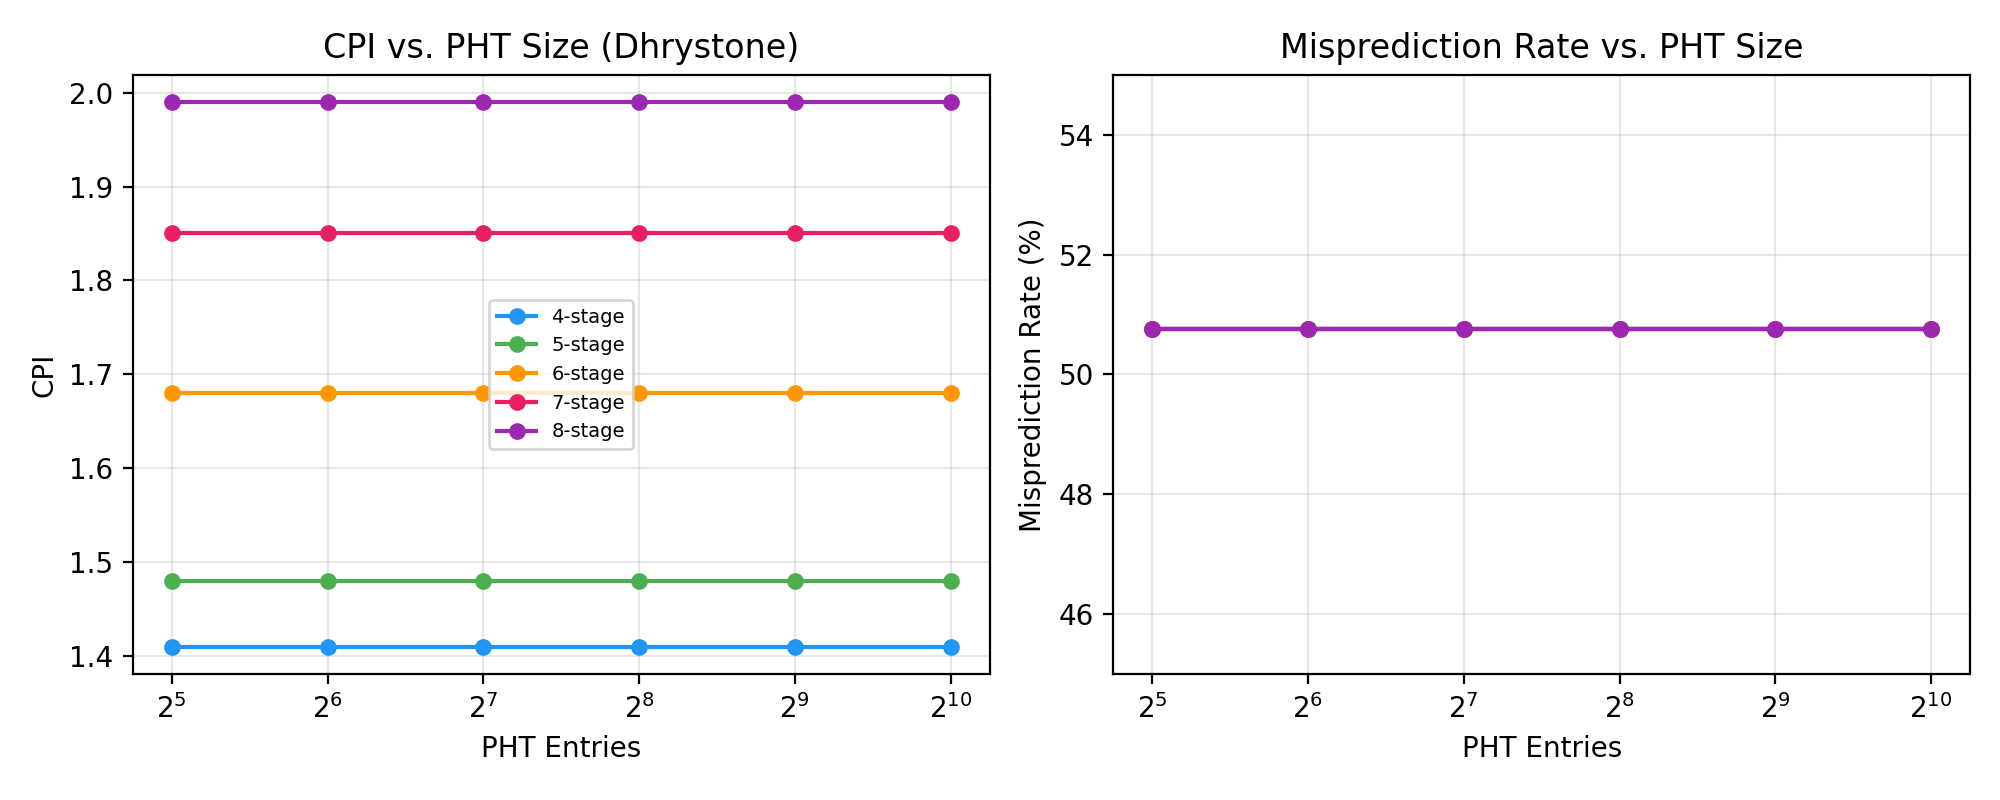
\includegraphics[width=\columnwidth]{predictor_sweep.png}
\caption{CPI and misprediction rate on Dhrystone across six PHT sizes (32--1024) and five pipeline depths (30 combinations). All 30 configurations yield identical misprediction counts (203), proving that Mechanism~B is orthogonal to predictor capacity.}
\label{fig:predsweep}
\end{figure}

\subsection{Gshare vs.\ Bimodal Comparison}
\label{sec:bimodal}

To establish generality across predictor architectures, we replaced the gshare predictor with a bimodal predictor that indexes the PHT using only the PC (no global history register) and ran Dhrystone on all five pipeline depths.
Fig.~\ref{fig:predarch} compares the two architectures.
The bimodal predictor produces nearly identical CPI values across all depths (4-stage: 1.41/1.41, 5-stage: 1.48/1.48, 6-stage: 1.68/1.68, 7-stage: 1.85/1.85, 8-stage: 1.99/1.99 for gshare/bimodal) and misprediction counts (202 vs.\ 203).
The CPI trend across pipeline depths is preserved regardless of whether the predictor uses global history correlation or purely local PC-based prediction.

SGF targets GHR-based predictors (gshare, TAGE, and similar correlation predictors).
For bimodal predictors, the analogous staleness effect would require speculative PHT forwarding, which is a different mechanism.
The prevalence of history-based predictors in modern designs makes SGF broadly applicable.

\begin{figure}[t]
\centering
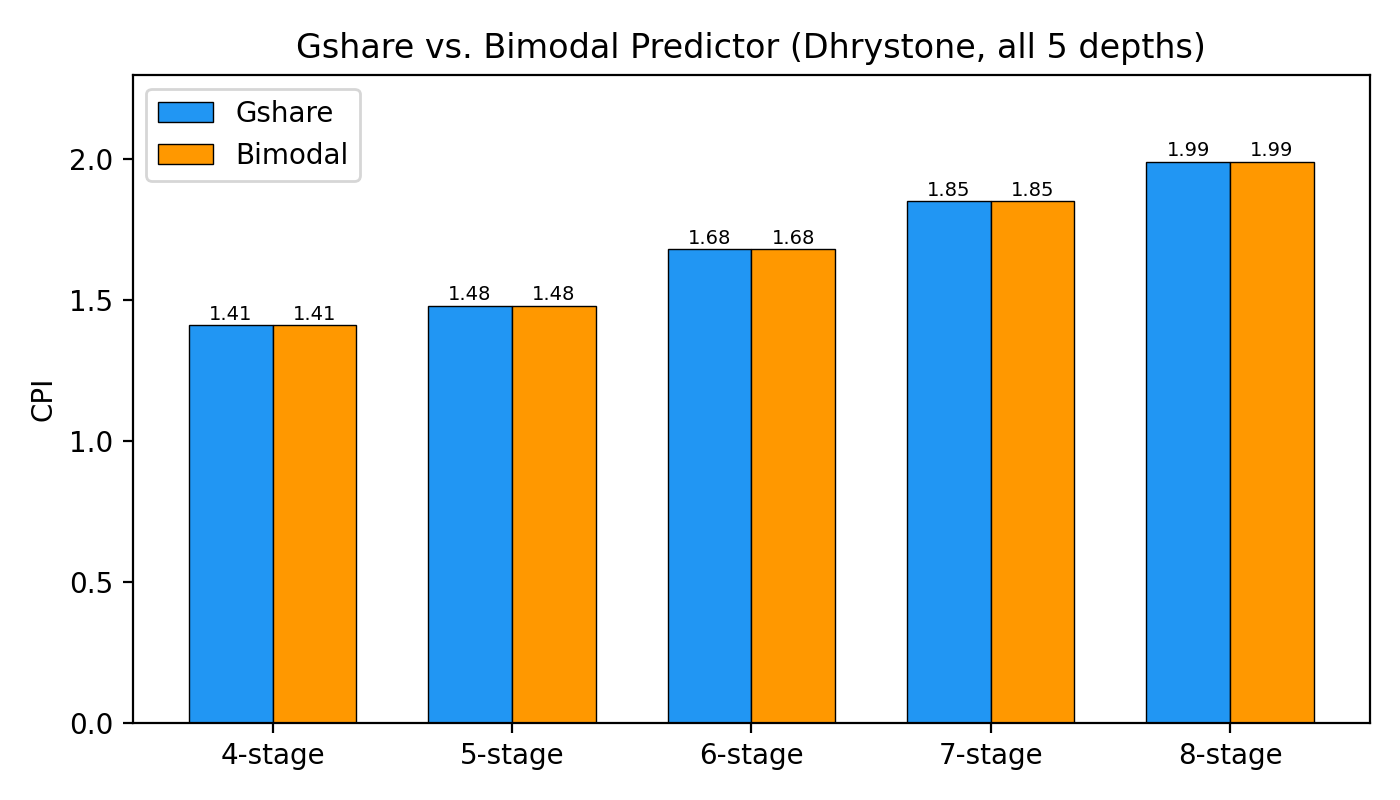
\includegraphics[width=\columnwidth]{predictor_architecture.png}
\caption{CPI comparison between gshare and bimodal predictors on Dhrystone. The pipeline-depth CPI trend is preserved across predictor architectures.}
\label{fig:predarch}
\end{figure}

\subsection{BRAM Instruction Memory Effect}
\label{sec:bram}

To test whether the 7-stage IF split becomes beneficial with synchronous memory, we synthesized BRAM variants of the 4-, 5-, 6-, and 7-stage pipelines using a registered-output instruction memory that infers Block RAM.
The 8-stage BRAM variant failed to route in Vivado due to congestion from the combined MEM1/MEM2 split and BRAM read-port timing; this routing failure is itself informative, as it indicates that the 8-stage memory split creates placement pressure that the Artix-7 fabric cannot resolve with BRAM-based instruction memory.
Fig.~\ref{fig:bram} shows the results for the four variants that completed successfully.

With BRAM, the 4-stage achieves 69.3\,MHz, the 5-stage 73.7\,MHz, the 6-stage 121.5\,MHz, and the 7-stage 120.9\,MHz.
The 7-stage design improves from 115.0\,MHz (LUT) to 120.9\,MHz (BRAM), nearly matching the 6-stage.
The 4-stage slightly decreases from 70.4 to 69.3\,MHz because the BRAM's registered output adds latency to the already-long execute-stage critical path.
The IF1/IF2 boundary naturally absorbs the BRAM's 1-cycle read latency, and the 7-stage becomes competitive with the 6-stage on frequency.
However, the CPI overhead of the deeper pipeline remains, so the 7-stage would need SGF and moderate-branch-density workloads to match the 6-stage's throughput even with BRAM-competitive frequency.

\begin{figure}[t]
\centering
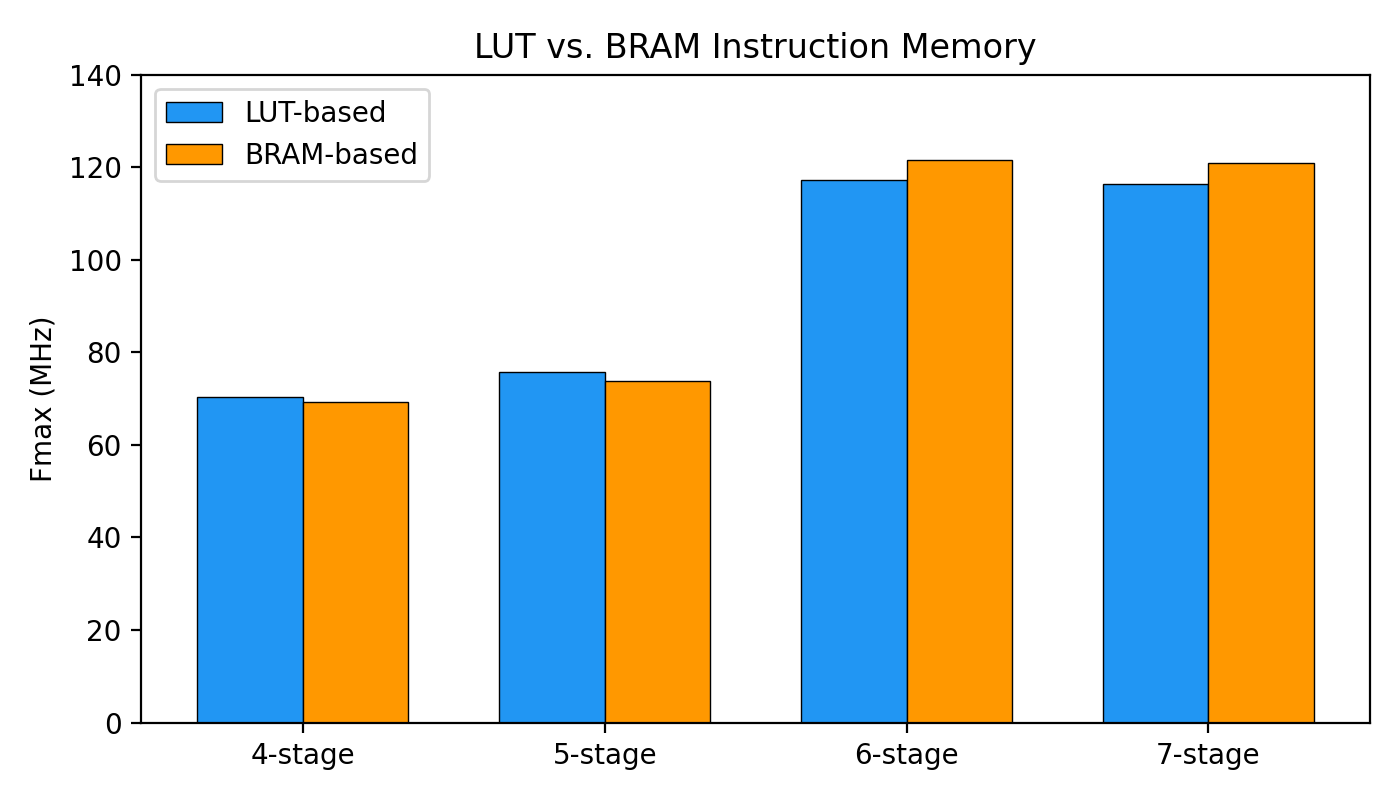
\includegraphics[width=\columnwidth]{bram_comparison.png}
\caption{$F_{\max}$ comparison between LUT-based and BRAM-based instruction memory for three pipeline depths on Artix-7.}
\label{fig:bram}
\end{figure}

\subsection{Power and Efficiency}
\label{sec:power}

Power estimates are obtained from SAIF-annotated switching activity analysis in Vivado for all five pipeline variants.
Fig.~\ref{fig:power} shows the on-chip power breakdown.
Total power ranges from 0.298\,W (6-stage) to 0.317\,W (8-stage), a spread of only 6\% across the full depth range.
Static power is constant at 0.069\,W across all variants.
Dynamic power increases modestly from 0.230\,W (5/6-stage) to 0.248\,W (8-stage), reflecting the additional pipeline registers and forwarding paths in deeper designs.

\begin{figure}[t]
\centering
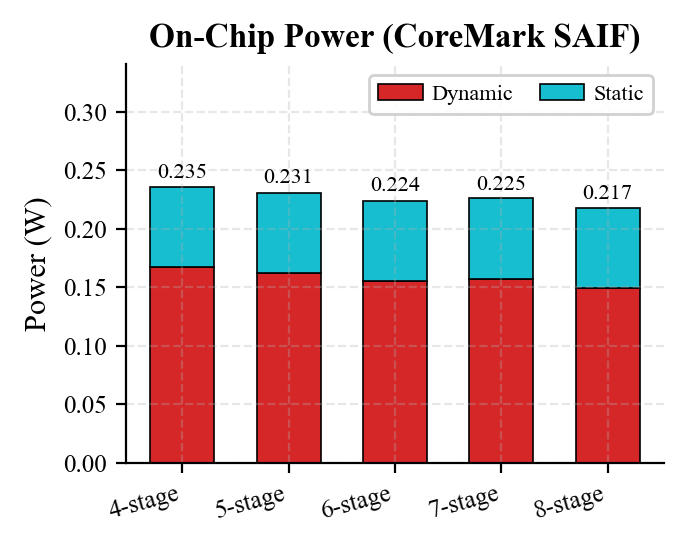
\includegraphics[width=\columnwidth]{power_comparison.png}
\caption{On-chip power breakdown (dynamic and static) for all five pipeline depths on Artix-7 (SAIF-based analysis).}
\label{fig:power}
\end{figure}

\textbf{Energy-Delay Product (EDP).}
To evaluate the power-performance tradeoff, we compute the energy per CoreMark execution and the EDP:
\begin{equation}
E = P_{\text{dyn}} \times \frac{\text{Cycles}}{F_{\max}}; \quad \text{EDP} = E \times \frac{\text{Cycles}}{F_{\max}}
\end{equation}
The 6-stage achieves the lowest energy (10.4\,mJ) and EDP (471\,mJ$\cdot$ms), beating the 4-stage (15.0\,mJ, 952\,mJ$\cdot$ms) by 50\% on EDP despite consuming similar power.
The 8-stage's energy rises to 13.4\,mJ due to higher CPI, yielding an EDP of 718\,mJ$\cdot$ms.
The 6-stage is the most energy-efficient depth on this fabric because its 67\% frequency advantage over the 4/5-stage outpaces the 4\% power increase.
SGF's additional 55 LUTs and 63 FFs add $<$1\% to dynamic power (estimated from the resource proportion), confirming negligible energy overhead.

Fig.~\ref{fig:efficiency} shows the power efficiency in MIPS per watt across all five depths.
The 6-stage leads at 237\,MIPS/W, followed by the 7-stage at 203\,MIPS/W and the 4-stage at 168\,MIPS/W.
The 5-stage (155\,MIPS/W) and 8-stage (166\,MIPS/W) are the least efficient, confirming that the 5-stage is a dominated design point on power efficiency as well as throughput.

\begin{figure}[t]
\centering
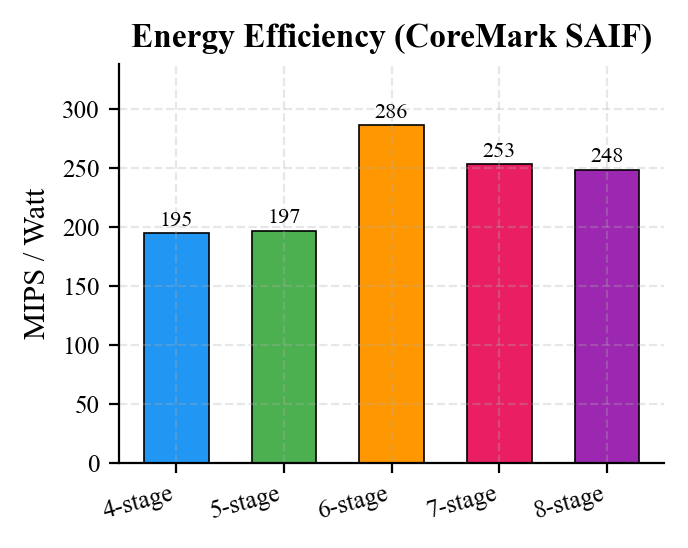
\includegraphics[width=\columnwidth]{efficiency_comparison.png}
\caption{Power efficiency (MIPS/W) for all five pipeline depths (SAIF-based power, diagnostic workload throughput).}
\label{fig:efficiency}
\end{figure}

\subsection{Published Cores Context}
\label{sec:published}

Fig.~\ref{fig:published} places our five variants alongside published RISC-V soft cores on Artix-7 as a \emph{sanity check}---confirming that the research vehicle occupies a realistic region of the design space.
Our variants sit in the mid-range.
Higher-frequency cores (SERV at 300\,MHz \cite{serv2019}, PicoRV32 at 250\,MHz \cite{picorv32}) use bit-serial or multi-cycle execution that eliminates pipelined forwarding paths.
These cores are not directly comparable because they differ in ISA support, predictor design, and forwarding philosophy---precisely the confounding variables our experiment controls.

\begin{figure}[t]
\centering
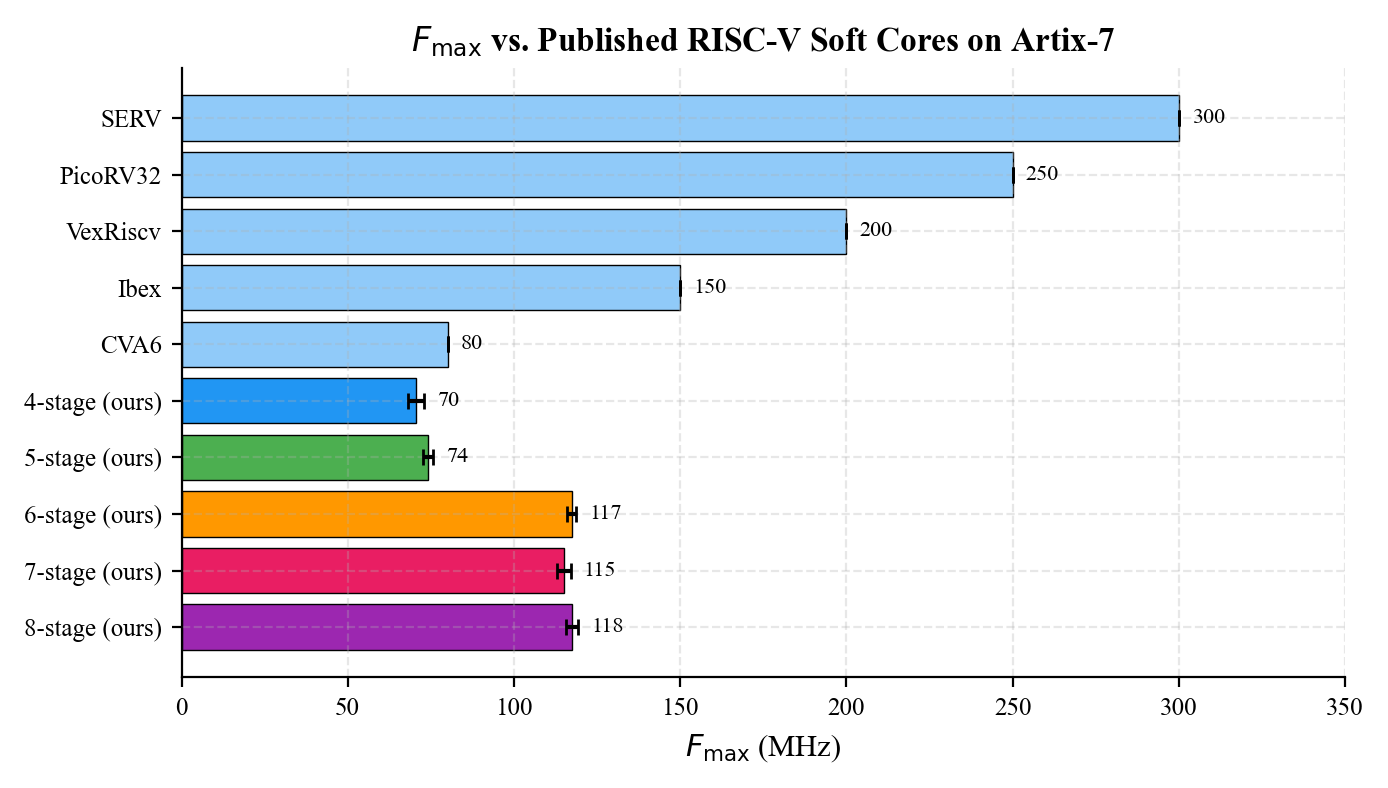
\includegraphics[width=\columnwidth]{published_cores_comparison.png}
\caption{$F_{\max}$ comparison with published RISC-V soft cores on Artix-7. Our variants (highlighted) occupy a realistic mid-range; direct performance comparison is not meaningful because the published cores differ in ISA support, predictor design, and forwarding philosophy.}
\label{fig:published}
\end{figure}

% ====================================================================
\section{Limitations}
\label{sec:limitations}
% ====================================================================

The boundaries of this study constrain every conclusion drawn above and must be stated precisely.

\textbf{Single fabric.}
The primary platform is Xilinx Artix-7 XC7A35T with Vivado 2025.2.
Absolute $F_{\max}$ values and the exact location of the execute-split frequency knee are fabric-specific.
Intel ALM-based devices and non-Xilinx synthesis tools remain untested.

\textbf{Single microarchitecture.}
The processor is a research vehicle, not a production-competitive core.
It lacks compressed-instruction support, out-of-order execution, cache hierarchy beyond a single L1, and I/O subsystems.
Results characterize how \emph{this particular} microarchitecture responds to pipeline-depth changes.
A core with a different forwarding topology, a tournament predictor, or a deeper memory hierarchy could produce a different optimal depth.

\textbf{Memory hierarchy scope.}
All workloads fit within 16\,KB of instruction memory with near-100\% cache hit rates.
The cache miss sensitivity analysis in Section~\ref{sec:cache_miss} bounds SGF's benefit under higher miss rates.

\textbf{CPI model per-workload parameters.}
The first-principles model (Eq.~\ref{eq:cpi_model}, $R^2 = 0.977$) decomposes CPI into physically meaningful terms but relies on per-workload $\gamma_w$ parameters that must be fitted empirically.
The model predicts the depth-dependent CPI components from architectural parameters alone; the workload-dependent base requires simulation or profiling.

\textbf{SGF predictor scope.}
SGF targets GHR-based predictors (gshare and its derivatives).
Extension to tournament or TAGE predictors, which maintain multiple history lengths, would require per-table speculative histories.
The crc32 marginal disbenefit (+167 mispredictions, +0.096\% absolute) demonstrates that SGF is not universally positive, though the effect is negligible.

% ====================================================================
\section{Conclusion}
\label{sec:conclusion}
% ====================================================================

This paper presents Speculative GHR Forwarding (SGF), a lightweight dual-GHR microarchitectural mechanism that eliminates stale-GHR branch-prediction degradation in deep FPGA pipelines.
SGF reduces mispredictions by 31.4\% on CoreMark and 22.7\% on statemate in 7-stage pipelines on Artix-7, at a cost of 0.5--0.7\% area with no $F_{\max}$ degradation.
The mechanism pushes deep-pipeline misprediction counts below the shallow-pipeline baseline because the speculative GHR reflects a more accurate approximation of the true branch history than any committed GHR operating with nonzero update latency.

SGF was motivated by controlled measurements that no prior work had performed.
Five RV32IM pipeline variants (4 through 8 stages), sharing identical RTL on Artix-7, were synthesized across 50 post-place-and-route runs and evaluated on seven benchmark workloads (35 validated data points).
The measurements revealed a two-tier frequency structure ($p < 10^{-48}$, Cohen's $d = 18.5$) and separated pipeline-depth CPI overhead into Mechanism~A (inherent penalty scaling) and Mechanism~B (correctable stale-GHR inflation).
A first-principles analytical model achieves $R^2 = 0.977$ across all data points, with physically interpretable terms for branch flush, load-use stalls, and IF2 bubbles.

For practitioners designing RV32IM-class soft cores on Artix-7: the 6-stage pipeline is the highest-throughput depth in this configuration, the classic 5-stage is a dominated design point, and any pipeline with 3 or more stages of predictor update latency should implement SGF.
The 0.5--0.7\% area cost is negligible; the 17--31\% misprediction reduction is not.

Future work includes extending SGF to tournament and TAGE predictor architectures, where multiple history lengths require per-table speculative state, and validating the two-tier frequency structure and SGF benefits on Intel FPGA fabrics.

The complete RTL, testbenches, synthesis scripts, and benchmark programs are publicly available at \url{https://github.com/devanshjoshi08/RISCV-RV32IM-Processor}.

% ====================================================================
% References
% ====================================================================

\bibliographystyle{IEEEtran}
\bibliography{references}

\end{document}
